\documentclass{iopart}
%\documentclass[showpacs,amssymb,prd,superscriptaddress,nofootinbib,amssymb,amsmath,amsfonts,aps,mathrsfs,altaffilletter]{revtex4-1}
%\documentclass[12pt]{article}

\usepackage{url}
\usepackage{amsbsy}
\usepackage{graphicx}
\usepackage{subfig}
\usepackage{graphicx}
\usepackage{graphicx,epsf, epsfig, amssymb}% Include figure files
\usepackage{bm}
%\usepackage{longtable}
\usepackage{url}
\usepackage{hyperref}
\usepackage{float}


\input{epsf}


%% Commands Alberto

\newcommand{\beq}{\begin{equation}}
\newcommand{\eeq}{\end{equation}}
\newcommand{\bes}{\begin{subequations}}
\newcommand{\ees}{\end{subequations}}
\newcommand{\bea}{\begin{eqnarray}}
\newcommand{\eea}{\end{eqnarray}}
\newcommand{\ba}{\begin{array}}
\newcommand{\ea}{\end{array}}
\newcommand{\beqn}{\begin{eqnarray*}}
\newcommand{\eeqn}{\end{eqnarray*}}
\newcommand{\dps}{\displaystyle}        
\newcommand{\p}{\partial}
\newcommand{\f}[2]{\frac{#1}{#2}}
\newcommand{\lisa}{{\em LISA}}
\def\ii{{\rm i}}   
\def\lappreq{\!\stackrel{\scriptscriptstyle <}{\scriptscriptstyle\sim}\!}
\def\gappreq{\!\stackrel{\scriptscriptstyle >}{\scriptscriptstyle\sim}\!}
\newenvironment{itemize_estret}{
\begin{itemize}
  \setlength{\itemsep}{1pt}
  \setlength{\parskip}{0pt}
  \setlength{\parsep}{0pt}
}{\end{itemize}}
\def\lappreq{\! \stackrel{\scriptscriptstyle <}{\scriptscriptstyle
\sim}\!}
\def\gappreq{\!\stackrel{\scriptscriptstyle >}{\scriptscriptstyle \sim}\!}
\def\be{\begin{equation}}
\def\ee{\end{equation}}
\def\beq{\begin{eqnarray}}
\def\eeq{\end{eqnarray}}
\def\f{\frac}
\def\nn{\nonumber}

%% Command from Emanuele

\newcommand{\secintro}{I}
\newcommand{\secsetup}{II}
\newcommand{\secresults}{III}
\newcommand{\secconclusion}{IV}

\newcommand{\eb}[1]{{\textcolor{red}{\sf{EB: #1}} }}
\newcommand{\Vitor}[1]{{\textcolor{blue}{\sf{Vitor: #1}} }}

\newcommand{\lp}{\left(}
\newcommand{\rp}{\right)}
\newcommand{\lb}{\left[}
\newcommand{\rb}{\right]}
\newcommand{\Dta}{\Delta}
\newcommand{\omg}{\omega}
\newcommand{\Gma}{\Gamma}
\newcommand{\lmda}{\lambda}
\newcommand{\lgl}{\langle}
\newcommand{\rgl}{\rangle}
\newcommand{\bgaln}{\begin{align}}
\newcommand{\bgeq}{\begin{equation}}
\newcommand{\eiwv}{e^{i\omega V}}
\newcommand{\eimphi}{e^{-im\phi}}
\newcommand{\npt}{($n+2$)}
\newcommand{\onespc}{\hspace{7pt}}
\newcommand{\rmnum}[1]{\romannumeral #1}
\newcommand{\Rmnum}[1]{\expandafter\@slowromancap\romannumeral #1@}
\def\ph{\phi_{lmn}}
\def\Qlm{Q_{lmn}}





\begin{document}



\title
{First results of scientific performance for the design of ESA space based gravitational wave detector ({\it ELISA}) }

\author{The \emph{Science Performance Task Force (SPTF)}:
Pau Amaro-Seoane$^1$,
Sofiane Aoudia$^1$,
G\'erard Auger$^2$,
Stanislav Babak$^1$,
Emanuele Berti$^3$
Neil J. Cornish$^4$,
Jonathan Gair$^5$,
Ryan Lang$^6$,
Tyson Littenberg$^6$,
Sean McWilliams$^6$,
Oliver Jennrich$^7$,
Philippe Jetzer$^8$,
Ioannis Kamaretsos$^9$,
Antoine Klein$^8$,
Gijs Nelemans$^{10}$,
Frank Ohme$^1$,
Eric Plagnol$^2$,
Antoine Petiteau$^1$,
Edward K. Porter$^2$,
Emma Robinson$^1$,
B. S. Sathyaprakash$^9$,
Bernard Schutz$^1$,
Alberto Sesana$^1$,
Carlos Sopuerta$^{11}$,
Alessandro Spallicci$^{12}$,
Ira Thorpe$^6$,
Michele Vallisneri$^{13,14}$,
Alberto Vecchio$^{15}$,
Marta Volonteri$^{16}$
}

\address{$^1$ Max-Planck-Institut f\"ur Gravitationsphysik (Albert-Einstein-Institut), Am M\"uhlenberg 1, D-14476 Golm bei Potsdam, Germany}
\address{$^2$ APC, UMR 7164, Univ.\ Paris 7 Denis Diderot, 10, rue Alice Domon et Leonie Duquet, 75025 Paris Cedex 13, France}
\address{$^3$ University of Mississippi, USA}
\address{$^4$ Dept.\ of Physics, Montana State Univ., Bozeman, MT 59717, USA}
\address{$^5$ Inst.\ of Astronomy, Univ.\ of Cambridge, Madingley Rd., Cambridge, CB30HA, UK}
\address{$^6$ Gravitational Astrophysics Lab., NASA Goddard Space Flight Center, 8800 Greenbelt Rd., Greenbelt, MD 20771, USA}
\address{$^7$ European Space Agency}
\address{$^8$ Institute of Theoretical Physics, University of Zurich}
\address{$^9$ School of Physics and Astronomy, Cardiff Univ., 5, The Parade, Cardiff, CF243YB, UK}
\address{$^{10}$ Department of Astrophysics, Radboud University Nijmegen, The Netherlands}
\address{$^{11}$ Institute of Space Sciences (ICE-CSIC), Barcelona, Spain}
\address{$^{12}$ University of Orleans, France}
\address{$^{13}$ Jet Propulsion Laboratory, California Inst.\ of Technology, Pasadena, CA 91109, USA}
\address{$^{14}$ Theoretical Astrophysics, California Inst.\ of Technology, Pasadena, CA 91125}
\address{$^{15}$ School of Physics and Astronomy, Univ.\ of Birmingham, Edgbaston, Birmingham B152TT, UK}
\address{$^{16}$ University of Michigan}

\ead{Antoine.Petiteau@aei.mpg.de, porter@apc.univ-paris7.fr}


\begin{abstract}

This document collects the current results of science performance studies of potential configurations for the "new LISA".    

\end{abstract}



%Uncomment for PACS numbers title message

%\pacs{00.00, 20.00, 42.10}



% Uncomment for Submitted to journal title message

%\submitto{\JPA}\



% Comment out if separate title page not required

\maketitle

\tableofcontents

%%%%%%%%%%%%%%%%%%%%%%%%%%%%%%%%%%%%%
%                                                       Instrument                                                      %
%%%%%%%%%%%%%%%%%%%%%%%%%%%%%%%%%%%%%
\section{ Instrument configurations : noises, orbits and sensitivity }
\label{S:Instrument}
{\it ('section captain' : Antoine Petiteau)}


\subsection{Overview}
\label{SS:Inst:Overview}

During the "first phase" (before CDF), 6 configurations had been defined. The table \ref{T:Configs} gives a summary of their main characteristics and the induced noise levels.

\begin{table}[H]
\begin{center}
\begin{tabular}{|c|c|c|c|c|c|c|}
\hline
Configuration 				& C5 	& C4	 	& C3 	& C2 	& C1  	& HL1 	\\
\hline
Armlength ($\times 10^9 $ m) 	& 2 		& 3 		& 1		& 1		& 1 	  	&  1 - 1.6 		\\
Orbits					& analytic & analytic & analytic & $10^o$ & closest 	& $20^o$ \\
\hline
Diameter telescope (m) 		& 0.28 	& 0.25 	& 0.25	& 0.4		& 0.4 	&  0.25 	\\
Laser power (W) 			& 2	 	& 0.7 	& 0.7		& 2		& 0.05 	&  0.7 		\\
Acceleration system 			& DRS	& DRS 	& DRS	& DRS	& LPF$^{(1)}$	&  DRS 	\\
\hline
Acceleration ($ 10^{-48} f^{-2} \textrm{Hz}^{-1}$)  & 6	&  6	& 6	& 6	&  $8.2\left( 1 + {  1.8 \times 10^4 \over f^2 }  \right) ^ 2 $	&   6 \\  %2.54	\\
Shot noise ($ 10^{-38} f^{2}  \textrm{Hz}^{-1}$)  &  2.05 &  20.07 &  2.31 & 0.06$^{(2)}$  & 4.92 & 2.31 \\ %11.2 \\
Fixed noise ($10^{-38} f^{2} \textrm{Hz}^{-1}$)  &  2.81 &  2.81 &  2.81 & 2.81  & 2.81 &  2.81 \\ %6.32 \\
\hline
\end{tabular}
\end{center}
\caption{Summary of configuration. Noises are given in $\delta \nu / \nu$ unit. \\ 
{ \scriptsize Notes about particular cases including mistakes : ${(1)}$ the margin has been taken into account 2 times  ; 
${(2)}$ the laser power has been considered in the rms shot noise  with power -1 instead of -0.5 . } }
\label{T:Configs}
\end{table}%


\subsection{Noises}
\label{SS:Inst:Noises}
The noise models used for the new space-based gravitational wave detector supported by ESA have been provided by ESA.
Each noise includes the standard ESA margin $M_{ESA} = 1 / 0.65 $ .

In the following description, we give the general formulation of the root mean square value (RMS), i.e. square root of the power spectral density (PSD) in the standard unit of the noise. 
We also give the value used for each configurations in relative frequency unit $\delta \nu \over \nu$.

The conversion between rms noise, $\delta x$,  and power spectral density $S$ is : $S = \delta x ^ 2$.

The conversion between acceleration noise unit (in $\textrm{m}^2.\textrm{s}^{-4}.\textrm{Hz}^{-1}$) and noise in length unit (in $\textrm{m}^2.\textrm{Hz}^{-1}$) is :
\begin{equation}
S(f) =  S_{\textrm{m}^2.\textrm{s}^{-4}.\textrm{Hz}^{-1}}(f) / (2 \pi f)^4 \;  \textrm{m}^2.\textrm{Hz}^{-1}
\end{equation}
 
The conversion between  noise in length unit ($\textrm{m}^2.\textrm{Hz}^{-1}$) and noise in relative frequency unit (in $\textrm{Hz}^{-1}$) is :
\begin{equation}
S_{\delta \nu \over \nu}(f) =  S (f) \times \left( {2 \pi f \over c } \right)^2 \;  \textrm{Hz}^{-1}
\end{equation}

 

\subsubsection{Acceleration noises}
\label{SSS:Inst:Noises:Acc}
This noise is due to the limitation of the drag-free system. 
We consider two types of acceleration noise : 
\begin{itemize}
\item DRS : acceleration noise corresponding to LISA requirements :
\begin{equation}
\delta x_{\textrm{acc}}^{\textrm{DRS}} =  M_{ESA} \times 3 \times 10^{-15}  \textrm{m}/\textrm{s}^2/\sqrt{\textrm{Hz}} 
\end{equation}

\item LPF  : acceleration noise corresponding to LISAPathfinder :
\begin{equation}
\delta x_{\textrm{acc}}^{\textrm{LPF}} = M_{ESA} \times 3.5 \times 10^{-15} \left( 1 + { 0.18 \ \textrm{mHz} \over f }  \right) \textrm{m}/\textrm{s}^2/\sqrt{\textrm{Hz}}
\end{equation}

\end{itemize}

So, we have one best case, the DRS, and one worth case, the LPF. 

Note that for the LPF noise, we include the ESA margin but, according to Stefano Vitale, the margin was already taken into account in the   $3.5 \times 10^{-15}$ value. So the LPF acceleration was over-estimated (only used for configuration C1).

The acceleration noise for the different configurations is :
\begin{itemize}
\item for C1 : 
\begin{equation}
S_{acc, {\delta \nu \over \nu}} (f)  =  8.17 \times 10^{-48} \left( { 1 \over f} + \left({1.8 \times 10^{-4} \over f ^2} \right) \right)^2 Hz^{-1}
\end{equation}
\item for C2, C3, C4, C5, HL1 :
\begin{equation}
S_{acc, {\delta \nu \over \nu}} (f)  =  6.00 \times 10^{-48} f^{-2} Hz^{-1}
\end{equation}
\end{itemize}
 






\subsubsection{Shot noise}
\label{SSS:Inst:Noises:Shot}

This noise depends directly on the received laser power after the travel between two spacecrafts. Therefore it depends on :
\begin{itemize}
\item $L$ : the armlength (in m ),
\item $D$ : the diameter of the telescope (in m),
\item $P$ : the emitted laser power (in Watt) 
\end{itemize}
 

\begin{equation}
\delta x,_{\textrm{SN}} = M_{ESA} \times  7.7 \times 10^{-12}  \left( {1 \ \textrm{W} \over P } \right)^{1/2} \left( { L \over 5 \times 10^9 \ \textrm{m}} \right) \left( {0.4 \ \textrm{m} \over D }\right)^2  \textrm{m}/\sqrt{\textrm{Hz}} 
\end{equation}


The acceleration noise for the different configurations is :
\begin{itemize}
\item for C1 : 
\begin{equation}
S_{SN, {\delta \nu \over \nu}} (f)  =  4.92 \times10^{-38} f^2 Hz^{-1}
\end{equation}
\item for C2 : 
\begin{equation}
S_{SN, {\delta \nu \over \nu}} (f)  =  6.14 \times10^{-40} f^2 Hz^{-1}
\end{equation}
\item for C3 : 
\begin{equation}
S_{SN, {\delta \nu \over \nu}} (f)  =  2.31 \times10^{-38} f^2 Hz^{-1}
\end{equation}
\item for C4 : 
\begin{equation}
S_{SN, {\delta \nu \over \nu}} (f)  =  2.07 \times10^{-37} f^2 Hz^{-1}
\end{equation}
\item for C5 : 
\begin{equation}
S_{SN, {\delta \nu \over \nu}} (f)  =  2.05 \times10^{-38} f^2 Hz^{-1}
\end{equation}
\item for HL1 : 
\begin{equation}
S_{SN, {\delta \nu \over \nu}} (f)  =  2.31 \times10^{-38} f^2 Hz^{-1}
\end{equation}
\end{itemize}



\subsubsection{Other measurement noises}
\label{SSS:Inst:Noises:OMS}

This noise groups to the perturbation of the optical path in the optical bench and the telescope and  the precision on the interference measurement by the photodiode and the phasemeter. 



\begin{equation}
\delta x_{\textrm{OMS}} = M_{ESA} \times 6.2 \times 10^{-12}   \textrm{m}/\sqrt{\textrm{Hz}} 
\end{equation}


The other measurement noise is the same for all the configurations :
\begin{itemize}
\item for C1,C2, C3, C4, C5, HL1 : 
\begin{equation}
S_{OMS, {\delta \nu \over \nu}} (f)  =  2.81 \times10^{-38} f^2 Hz^{-1}
\end{equation}
\end{itemize}


\subsubsection{Laser noise}
\label{SSS:Inst:Noises:Laser}

The laser noise which have a typical rms noise around 30 Hz.Hz$^-1/2$ is reduced by the Time Delay Interferometry method. 
For this study, we suppose that the application of TDI second generation reduce the laser noise below the other noise.
So it will not be consider.




\subsection{Orbits}
\label{SS:Inst:Orbits}
We use several spacecraft orbits divided in 2 types : LISA like orbits and Halo around Lagrange point L1.
There are 2 key points :
\begin{itemize}
\item the stability of the constellation which have implication to the mission duration and on the shot noise level (see \ref{SSS:Inst:Noises:Shot}).
\item the way of reaching the orbits which have direct budget link through the energy required 
\end{itemize}



\subsubsection{LISA like orbits}
\label{SS:Inst:Orb:LISA}
The LISA like orbits corresponds to  constellation in a pseudo-equilateral triangle. 
The barycenter of the constellation follows the Earth with a certain Earth-detector barycenter angle, $\theta_{EdB}$.
 For this type of orbits, the constellation 2 key points  are the armlength and the angle $\theta_{EdB}$.
 To keep the stability, if we want to increase the armlength, it implies an increase of  $\theta_{EdB}$ for limiting the tidal deformation due to the Earth.
 
 We test 2 orbits which are the output of numerical simulation done by Oliver Jennrich (ESA) : 
\begin{itemize}
\item  best case : $\theta_{EdB} = 10^o$ and $L = 10^9$ m,
\item worst case : closest to the Earth ($\theta_{EdB} = ??^o$) and $L = 10^9$ m,
\end{itemize}

We also use the standard analytical LISA orbits from \cite{dhu05} changing the armlength.

The figure \ref{F:OrbSC} shows the numerical orbits compared to the analytic orbits with $L = 10^9$ m.
Regarding the position of the spacecraft the numerical orbits are close to the analytic ones. This means that the analytic orbits are a good approximation to the numeric one for computing the response of the detector to gravitational waves.

\begin{figure}[H]
\begin{center}
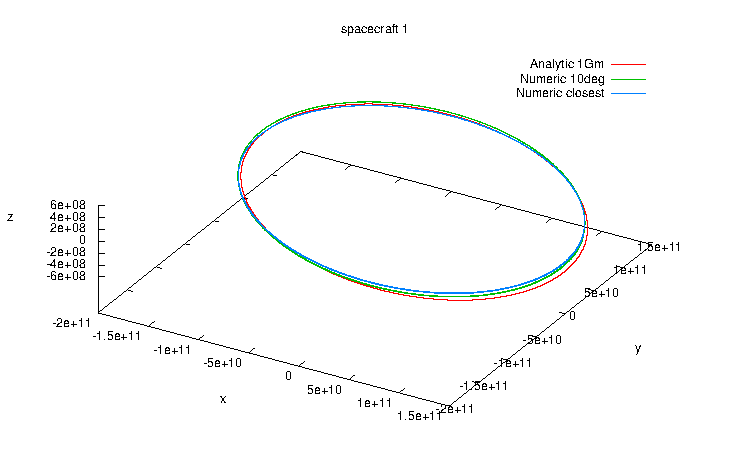
\includegraphics[width=0.45\textwidth]{FigNoiseOrbSens/Orb_SC1_LISA-CLISA-10LISA}
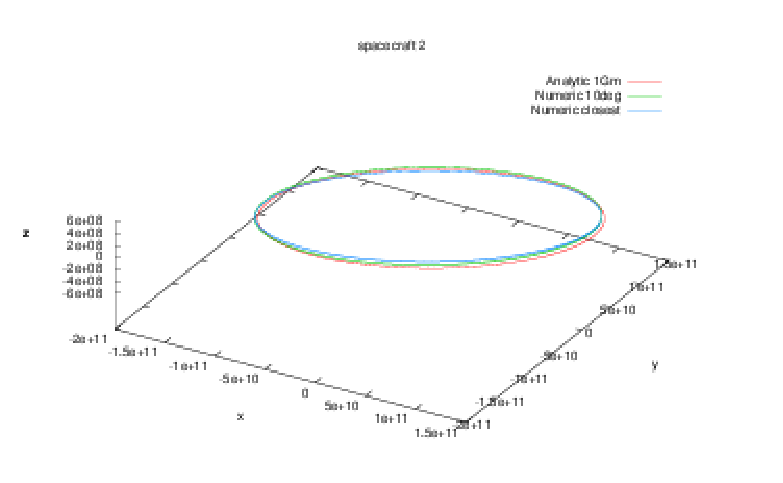
\includegraphics[width=0.45\textwidth]{FigNoiseOrbSens/Orb_SC2_LISA-CLISA-10LISA}
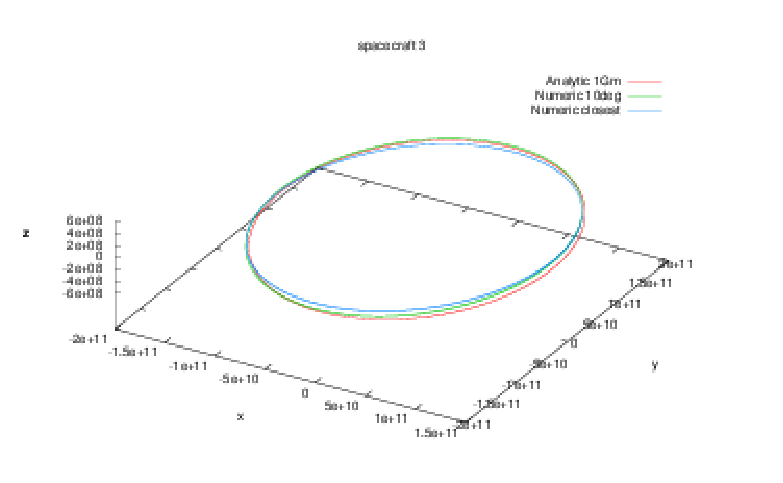
\includegraphics[width=0.45\textwidth]{FigNoiseOrbSens/Orb_SC3_LISA-CLISA-10LISA} 
\end{center}
\caption{Orbits of the 3 spacecrafts.
\label{F:OrbSC} } 
\end{figure}

The main difference between this orbits is the time variation of the armlength as shown on the figure \ref{Arm-1_LISA-CLISA-10LISA}.
This is an important point for the technological design of the detector (Doppler effect, ...) and for the application of the Time Delay Interferometry which is the pre-data-analysis method for reducing the laser noise. 

\begin{figure}[H]
\begin{center}
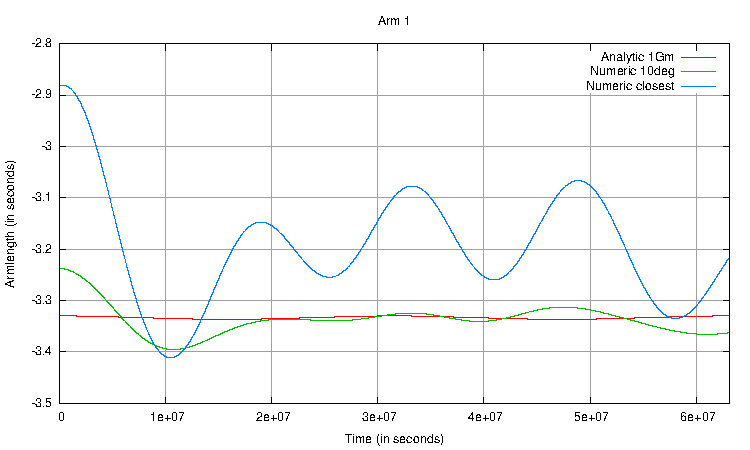
\includegraphics[width=0.45\textwidth]{FigNoiseOrbSens/Arm-1_LISA-CLISA-10LISA}
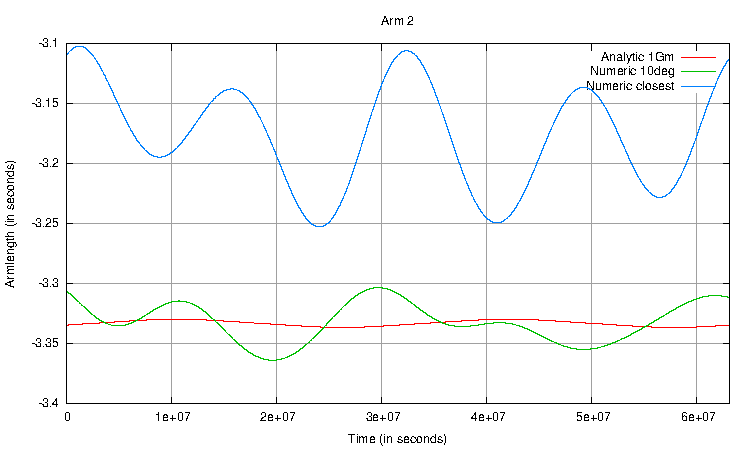
\includegraphics[width=0.45\textwidth]{FigNoiseOrbSens/Arm-2_LISA-CLISA-10LISA}
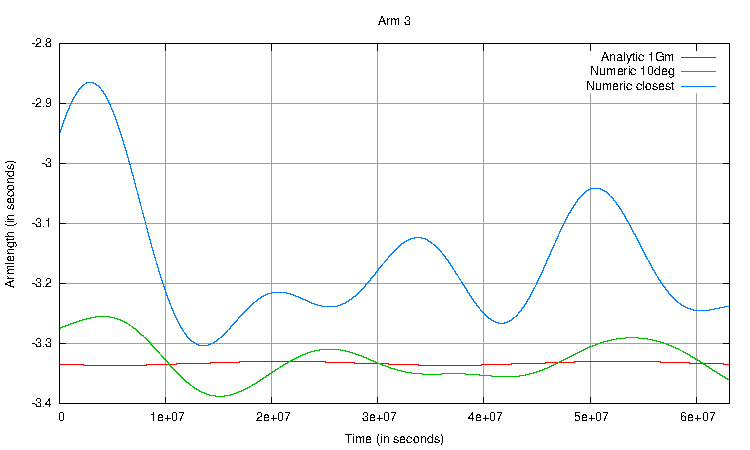
\includegraphics[width=0.45\textwidth]{FigNoiseOrbSens/Arm-3_LISA-CLISA-10LISA} 
\end{center}
\caption{Time evolution of the 3 armlength during 2 years.
\label{F:ArmEvol} } 
\end{figure}

\subsubsection{Halo around L1}
\label{SS:Inst:Orb:HL1}

We test another kind of orbits : the Halo around Lagrange point L1.
This orbits are the results of numerical simulation done by Vitali Mueller (AEI-Hannover).
It's a mother/daughter configuration : there are only 4 links (2 arms).
The figure \ref{F:HL1Orb} shows the orbits and the figure \ref{F:HL1Arm} shows the armlength evolution.

\begin{figure}[H]
\begin{center}
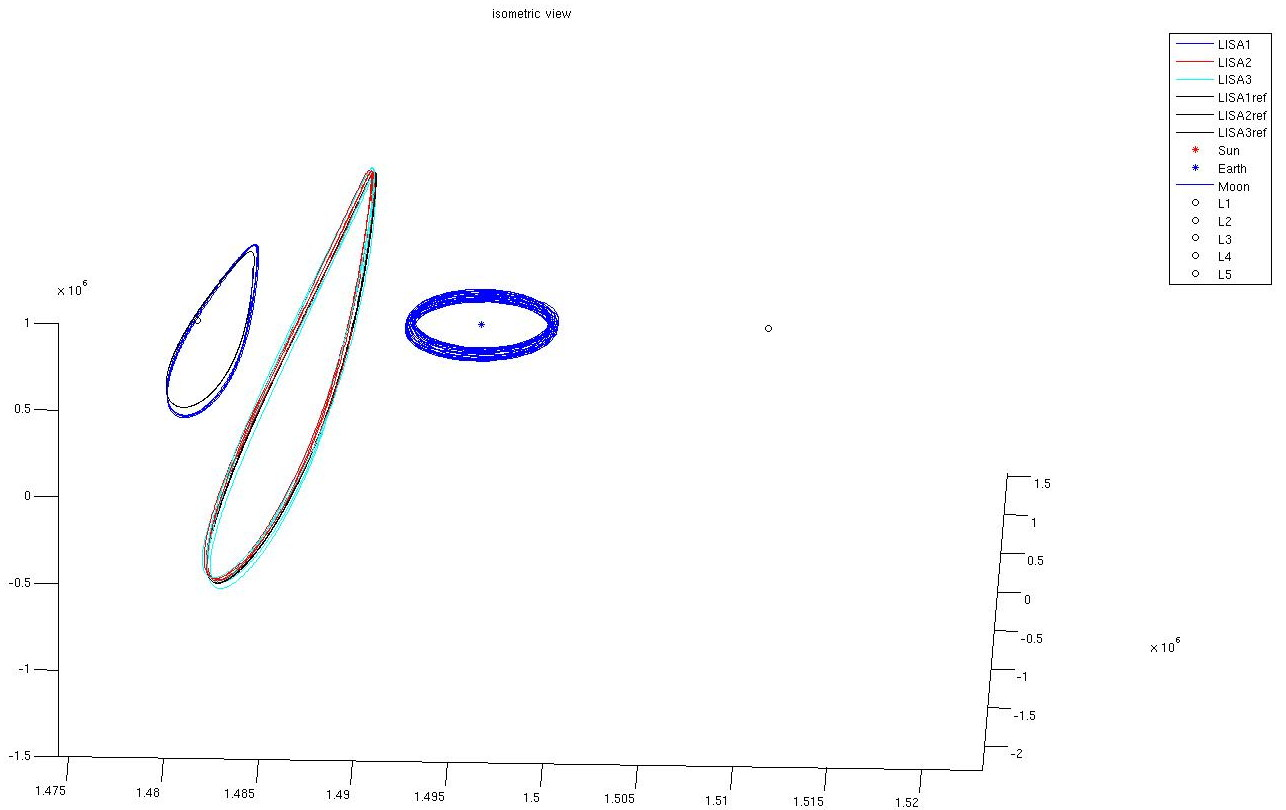
\includegraphics[width=\textwidth]{FigNoiseOrbSens/HL1isometric}
\end{center}
\caption{Orbits of spacecraft for the Halo around L1 configuration.
\label{F:HL1Orb} } 
\end{figure}

\begin{figure}[H]
\begin{center}
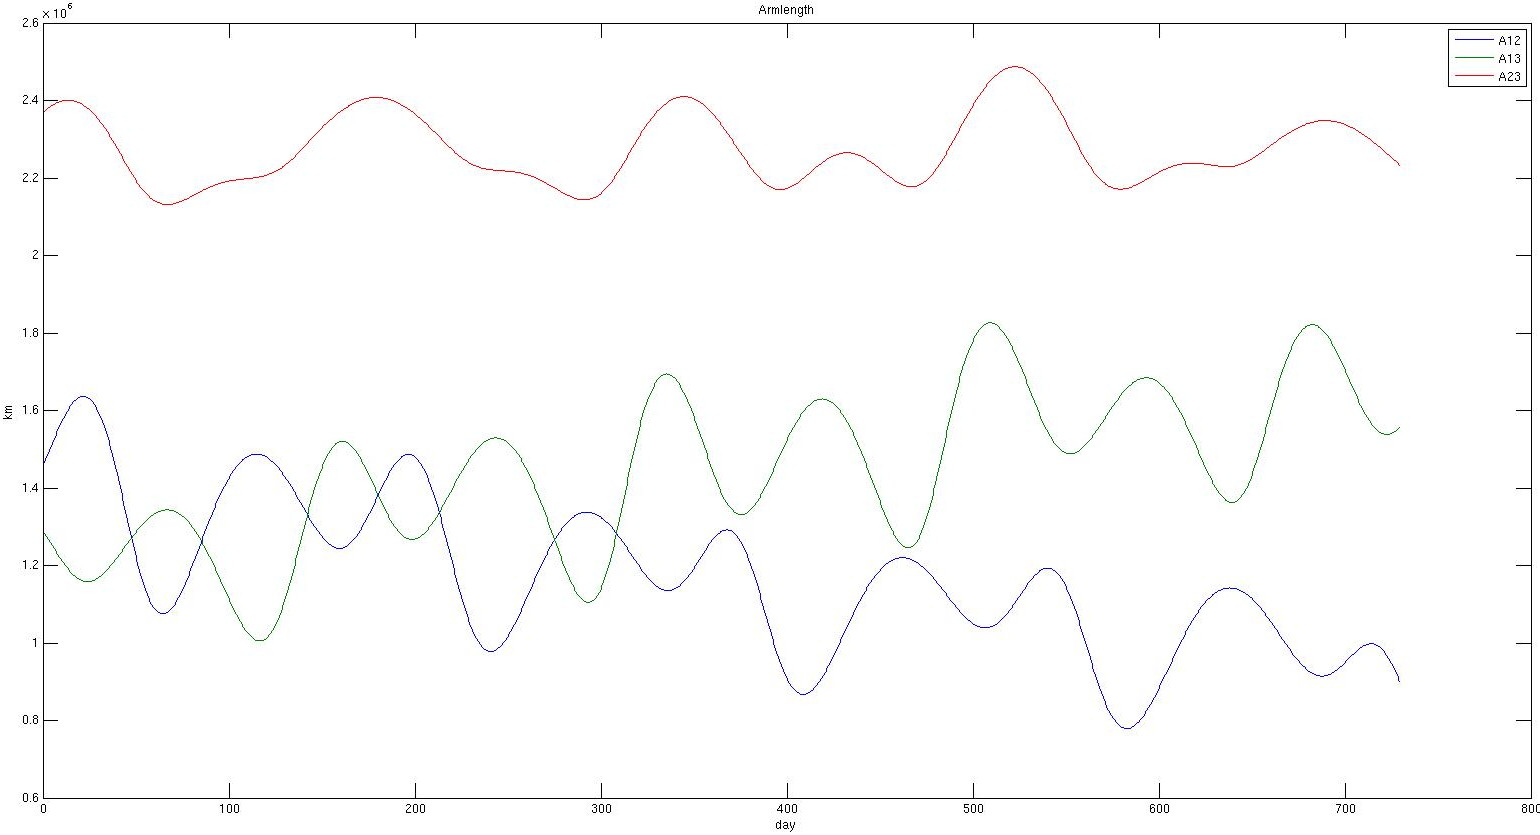
\includegraphics[width=\textwidth]{FigNoiseOrbSens/HL1armlength}
\end{center}
\caption{Evolution of armlength for the Halo around L1 configuration.
\label{F:HL1Arm} } 
\end{figure}



The main spacecraft (mother) is on a close orbit around L1 and the 2 daughters are on a distant orbits separated in phase by  $\pi$.
The angle between the 2 arms is around 120$^o$. The armlengths evolve between 1 and 1.6 million km.




\subsection{Noise power spectral density (PSD) }
\label{SS:Inst:PSD}


\subsubsection{Analytical model}
\label{SSS:Inst:PSD:Ana}

The  analytic formulation of the Power Spectral Density of TDI X can be approximated by (usual approximation used in LISA) : 
\begin{equation}
S^X_{n, {\delta \nu \over \nu}}(f) = 16 * \sin^2(\phi_L(f))  \left(  S_{SN, {\delta \nu \over \nu}}(f) + S_{OMN, {\delta \nu \over \nu}}(f) + \left( 3 + \cos(2 \phi_L(f) ) \right) S_{acc, {\delta \nu \over \nu}}(f) \right) 
\label{PSDXNoiseLISA}
\end{equation}
with $ \phi_L(f) =  2 \pi f L/c $

\begin{figure}[H]
\begin{center}
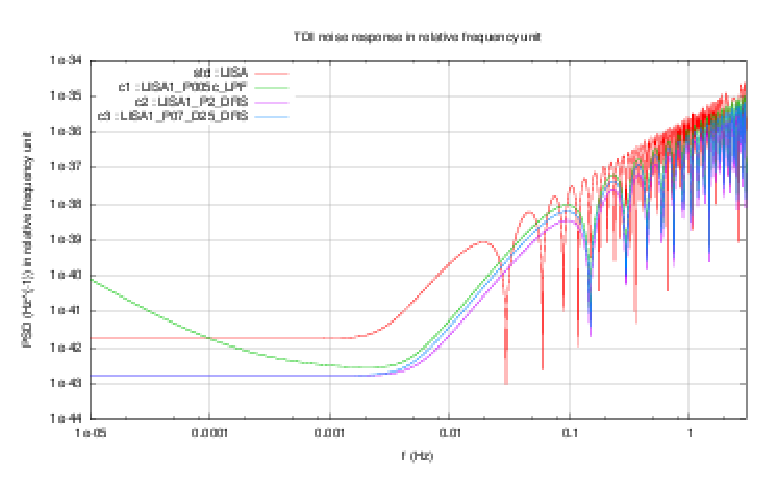
\includegraphics[width=0.9\textwidth]{FigNoiseOrbSens/PSD-Noise_std-c1-c2-c3}
\caption{Comparison of power spectral density of noises' response for  standard LISA, configurations 3a, 4a and 5a}
\label{F:PSDNoiseCompC3C4C5}
\end{center}
\end{figure}


\begin{figure}[H]
\begin{center}
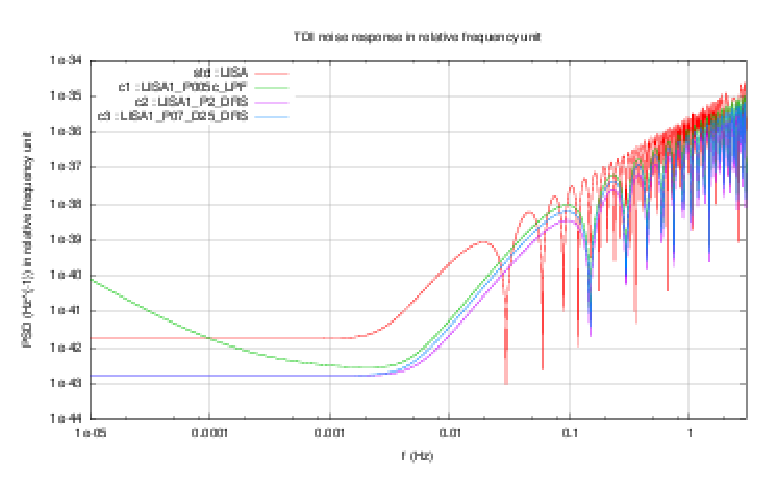
\includegraphics[width=0.9\textwidth]{FigNoiseOrbSens/PSD-Noise_std-c1-c2-c3}
\caption{Comparison of power spectral density of noises' response for standard LISA, configurations 1c, 2 and 3}
\label{F:PSDNoiseCompC1C2C3}
\end{center}
\end{figure}



\subsubsection{Simulation}
\label{SSS:Inst:PSD:Sim}






\subsection{Sensitivity}
\label{SS:Inst:Sensitivty}

\subsubsection{Analytical model}
\label{SSS:Inst:PSD:Ana}

(Very) approximative analytic formulation (based on LISA science requirements document (2010)) : 

The transfert function is 
\begin{equation}
T(f) = \sqrt{ 1 + \left( { f \over (0.41 \left({c \over 2 L} \right) )} \right)^2 }
\label{TransfertLISA}
\end{equation}

Sensitivity formulation :
\begin{equation}
\sqrt{S^{X}_h}(f) = \sqrt{5}  {2 \over \sqrt{3}} T(f)  { \sqrt{ 4 S_{acc} + S_{SN} + S_{omn} } \over L}
\label{AppSensXLISA}
\end{equation}


\begin{figure}[H]
\begin{center}
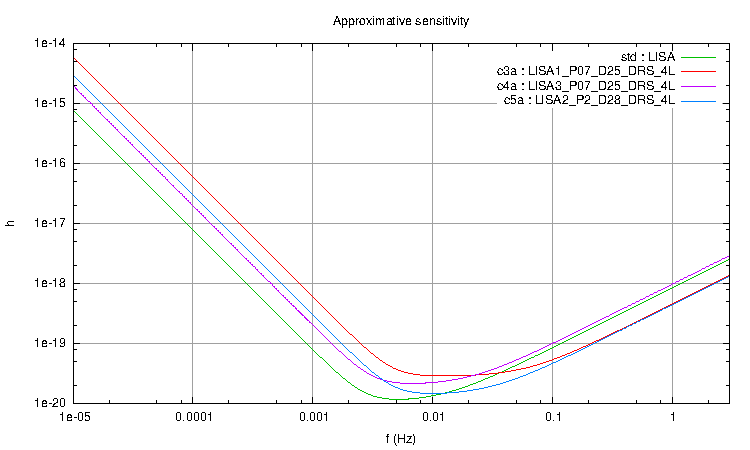
\includegraphics[width=0.9\textwidth]{FigNoiseOrbSens/Sensitivity_std-c3-c4-c5}
\caption{Comparison of sensitivity (SNR=1, "instantaneous") for standard LISA, configurations 3a, 4a and 5a}
\label{F:SensCompC3C4C5}
\end{center}
\end{figure}


\begin{figure}[H]
\begin{center}
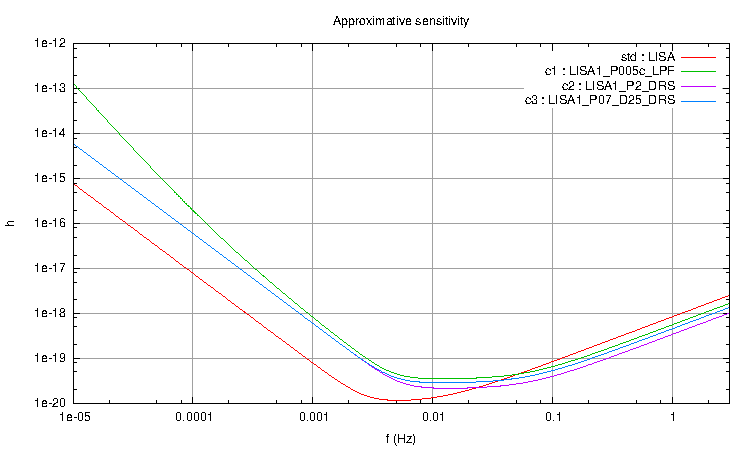
\includegraphics[width=0.9\textwidth]{FigNoiseOrbSens/Sensitivity_std-c1-c2-c3}
\caption{Comparison of sensitivity (SNR=1, "instantaneous") for standard LISA, configurations 1c, 2 and 3}
\label{F:SensCompC1C2C3}
\end{center}
\end{figure}


\subsubsection{Simulation}
\label{SSS:Inst:PSD:Sim}



%%%%%%%%%%%%%%%%%%%%%%%%%%%%%%%%%%%%%
%                                                 Galactic binaries                                                 %
%%%%%%%%%%%%%%%%%%%%%%%%%%%%%%%%%%%%%

\section{ Science return for Galactic Binaries }
\label{S:GalBin}
{ \it \small ('section captain' : Tyson Littenberg)}

Here we summarize the detection capabilities for Galactic Binaries with different ELISA configurations.

\subsection{Methodology}
The galactic confusion estimation is performed using the {\tt GB\_confusion} package of codes which have 
been incorporated into {\tt lisatools/MLDCwaveforms}.  Included in the directory on the SVN repository are 
example files, run scripts and a (readable?) README. 

To estimate the confusion noise we first simulate the instrument response to the galactic foreground by 
generating and co-adding waveforms for each source in the simulated galaxy downloaded from 
\begin{quotation}
{\tt https://lisa-light.aei.mpg.de/bin/view/GalacticBinaries/PopulationGalacticBinaries}
\end{quotation}  
The {\tt GB\_confusion} codes expect the source 
catalogue to be in the ``MLDC'' file format, i.e. with columns
\[f_0,\ \dot{f}_0,\ \theta,\ \phi,\ \mathcal{A}_0,\  \iota,\ \psi,\ \varphi_0. \]
Parameters $f$ is the GW frequency, subscript 0 denotes values measured at the start of the mission observation, $\{\theta,\phi\}$ are the 
ecliptic latitude and longitude of the source in radians, $\mathcal{A}$ is the amplitude, and $\{\i,\psi,\varphi_0\}$ are 
the inclination, polarization, and initial wave phase, together describing the orientation of the binary with respect 
to the line of sight from the solar system barycenter (SSB).  The{\tt PopulationGalacticBinaries} sources are parameterized 
by their orbital period (and $\dot{P}$), the component masses of the binary, the luminosity distance, and the sky-location in 
galactic coordinates, so the appropriate conversions need to be applied \emph{a priori}.  Also, the supplied galaxy simulations are over-populated with interacting binaries (those with $\dot{f}_0<0$ by a factor of $\sim10$.  We account for this by randomly
culling 90\% of mass-transferring binaries from the population before computing the instrument response.  While the TDI 
signals from the galaxy are being simulated, any binaries with signal-to-noise ratio (SNR) greater than one are stored in a 
separate ``Brights'' file which will later analyzed to determine which are detectable.

With the simulated data in hand, we iteratively estimate the confusion noise by dividing the Fourier domain data into $\sim30$ segments between $\sim10^{-4}$ and $\sim10^{-1}$ Hz and compute the median Fourier power in each segment.  The SNR for each signal in the Brights file is computed against this confusion noise (plus instrument noise), and any with signal-to-noise 
greater than 7 are stored as ``detectable'' and removed from the data.  This process is repeated iteratively until the confusion 
estimation converges.  The analysis is performed simultaneously considering 4- and 6-link configurations, producing separate 
results for the Michelson ``X'' channel (4 links) and noise orthogonal ``AET'' channels (6 links).

To understand the parameter estimation capabilities of different configurations, the lower-bound on the uncertainties for each source's parameters are computed using the Fisher Information Matrix (FIM), using the instrument + confusion noise as the weighting in the inner products.  We separately report on the number of  signals w/ $\dot{f}$ measured w/in 20\% as a 
proxy for number with measurable $D_L$.  Using only $\dot{f}$ to disentangle the distance from the overall amplitude 
implicitly assumes that the binary's dynamics are dominated by the radiation reaction force.  To unequivocally verify this assumption, we also need to measure the second time derivative of the frequency which was a difficult task even for LISA.  

\subsection{Results}
\subsubsection{Confusion Noise}
The confusion noise estimates for each configuration under consideration are shown in Figure~\ref{Figure:Confusion}.  The green [dashed] traces show the instrument noise.  The red [solid] curves are are the full noise spectra with confusion noise included, illustrating the impact of the astrophysical foreground on the instrument sensitivity.  The the black [dotted] lines are 
the LISA baseline instrument noise, and are included for reference.  All estimates are for two year observation 
times.  The confusion noise does not have a significant impact on the detector sensitivity for the 1 Gm configurations.
\begin{figure*}[H]
   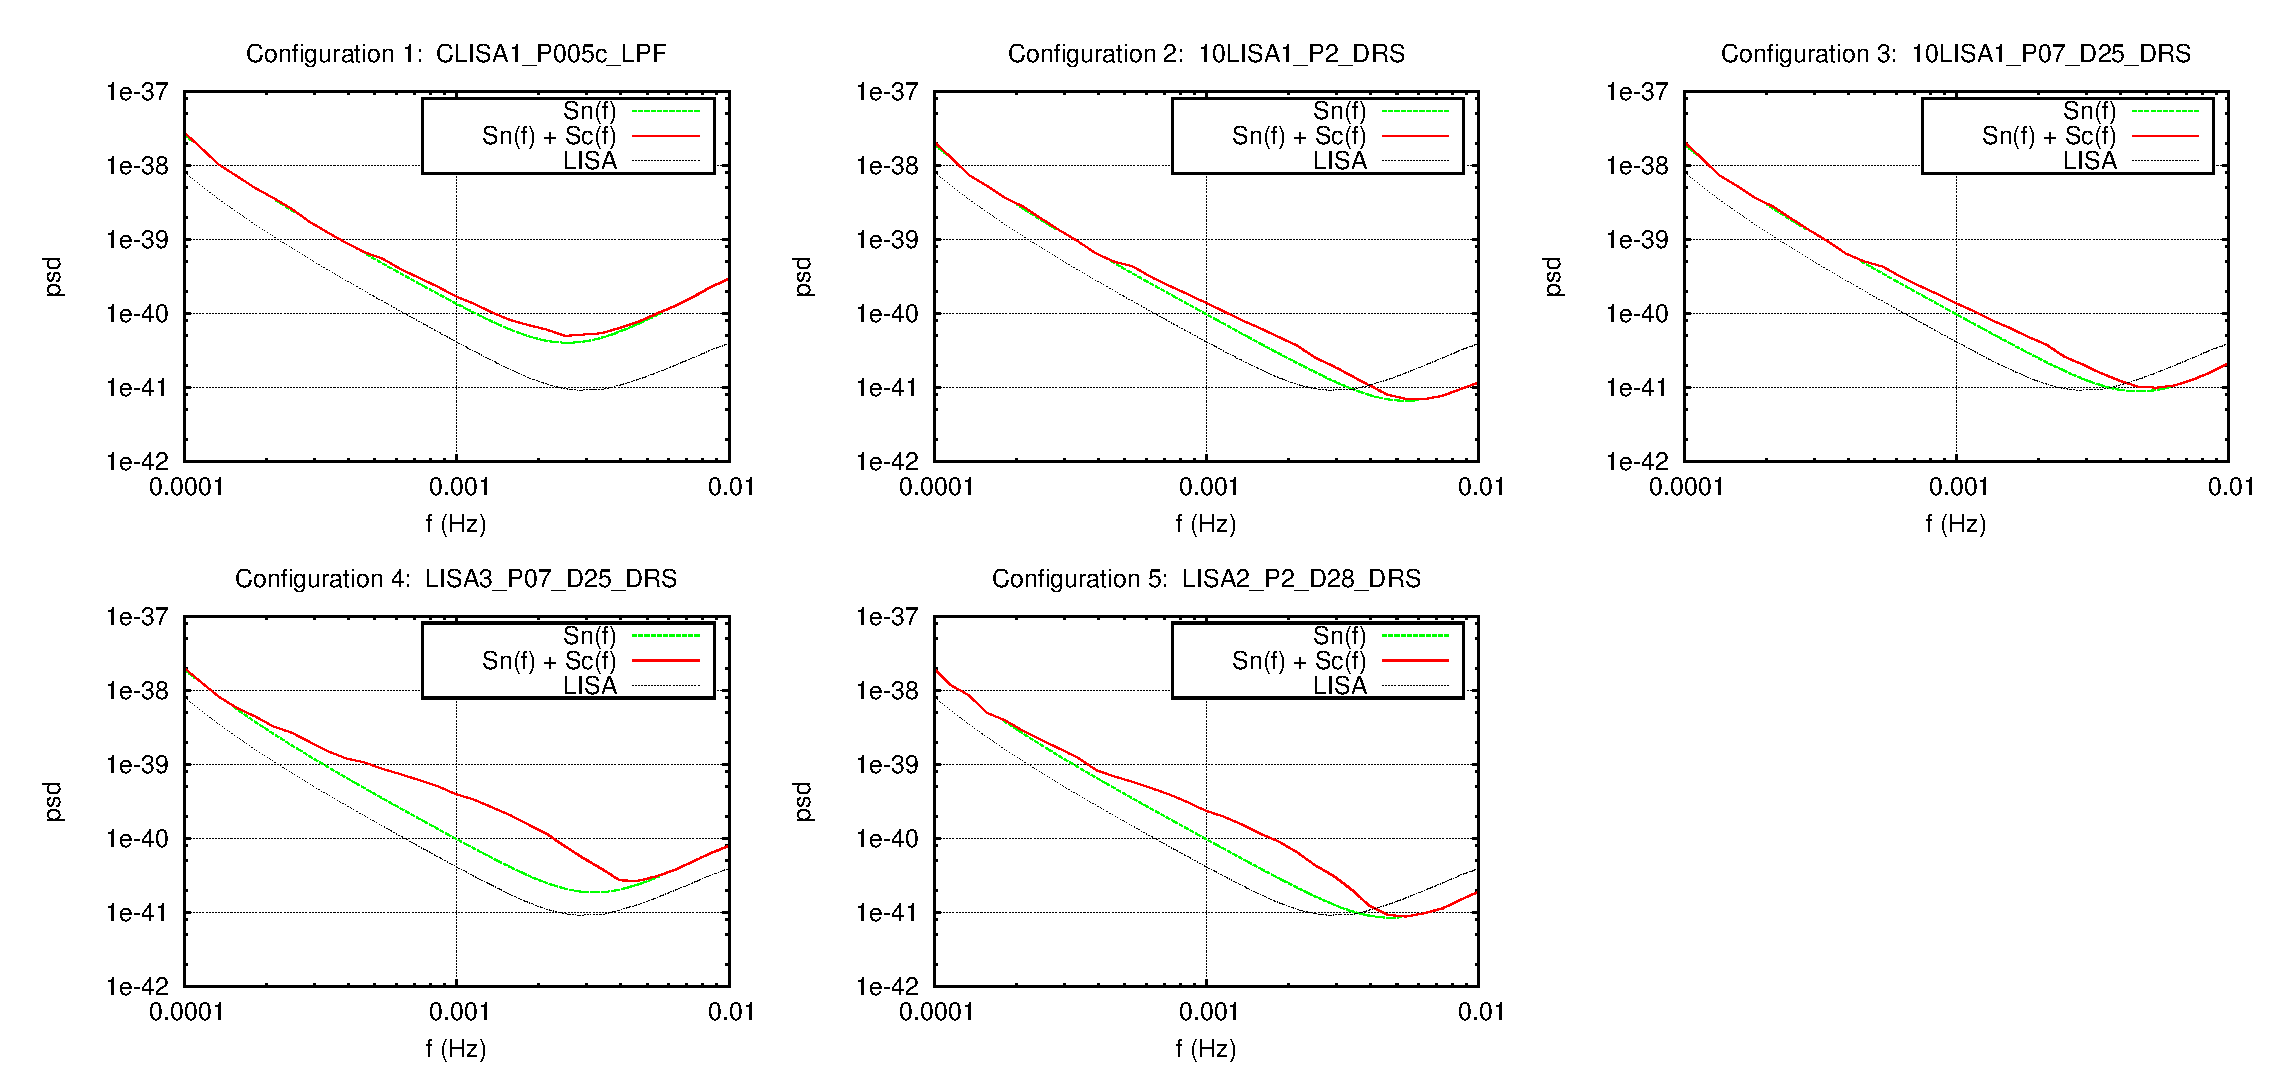
\includegraphics[width=1\textwidth]{confusion.eps} % requires the graphicx package
   \caption{Noise spectra for different detector configurations.  The red [solid] curves show the full noise spectrum, the green [dashed] curves are the instrument-only noise spectra and the black [dotted] line is the baseline LISA instrument noise curve.  All results are for two year mission lifetimes. }
   \label{Figure:Confusion}
\end{figure*}

\subsubsection{Recovered Source Catalogue}
Here we use the lists of detectable binaries and the FIM to make very coarse statements about the science potential for the 
different configurations.  Table~\ref{Table:Fisher} summarizes the parameter estimation results.  Of the total number of 
detectable binaries (shown in the SNR$>7$ column of the table), the number of which that can be resolved on the sky to 
$\lesssim$ 1 deg$^2$ are separately tabulated.  This number ranges between a few hundred to $\sim 2000$ for the most sensitive configuration.  Binaries with a fractional error in $\dot{f}_0$ of less than 20\% are of particular interest, as the 
frequency evolution can be used to constrain the luminosity distance to the source.  Perhaps the most astrophysically 
interesting number is in the final column of Table~\ref{Table:Fisher}, which shows the number of detectable binaries that are 
both well localized in the sky and have potentially well constrained luminosity distances.  It is from this sub-population of 
detectable binaries that the 3D spatial distribution of the Galaxy can be directly probed.  The bottom row of the table shows 
the results for the baseline LISA design.

The evaluation software also tracks the number of binaries with $\ddot{f}_0$ constrained to within 20\%.  This quantity is 
required to unambiguously determine if the orbital period of the binary is being solely driven by the emission of gravitational 
waves, or if there is some additional dynamical interaction between to two stars.  Unfortunately, for the new configurations 
being considered, only a few binaries will have sufficiently well constrained $\ddot{f}$ during a two year observation time.  This is not all that surprising, as the prospects for measuring  $\ddot{f}_0$ with LISA were uncertain at best.
\begin{table}[H]
\begin{center}
\begin{tabular}{cccccc}
\hline\hline
& Detector & SNR$>7$ & $\Delta \Omega \lesssim 1$ deg$^2$ & $\Delta\dot{f}/\dot{f} \leq 20\%$ & $\{\theta,\phi,D_L\}$\\
& Configurations & 4-link (6-link) & 4-link (6-link) & 4-link (6-link)  & 4-link (6-link)\\
\hline
1: &{\tt CLISA1\_P005c\_LPF} & 1071 (1846) & 149 (387) & 290 (469) & 33 (55)\\
2: &{\tt 10LISA1\_P2\_DRS} & 4586 (6204) & 1107 (1892 )& 1331 (1678) & 370 (457)\\
3: &{\tt 10LISA1\_P07\_D25\_DRS} & 4087 (5735) & 932 (1679) & 1176 (1510) & 286 (357)\\
4: &{\tt LISA3\_P07\_D25\_DR} & 7058 (12754) & 1527 (2997) & 1563 (2093) & 465 (616) \\
5: &{\tt LISA2\_P2\_D28\_DRS} & 6827 (11272) & 1821 (3150) & 1814 (2284) & 628 (814) \\
%-- &{\tt LISA} & -- & -- & -- & --\\
\end{tabular}
\caption{Summary of FIM parameter estimation results for the ensemble of detectable binaries for each configuration, 
considering both 6-link and 4-link operations.  All results are for two year mission lifetimes. }
\label{Table:Fisher}
\end{center}
\end{table}

\subsubsection{Verification Binaries}








%%%%%%%%%%%%%%%%%%%%%%%%%%%%%%%%%%%%%
%                                     Massive Black Hole binaries                                        %
%%%%%%%%%%%%%%%%%%%%%%%%%%%%%%%%%%%%%

\section{ Massive Black Hole binaries}
\label{S:MBHb}





%%%%%%%%%%%%%%%     MBHb : Population
\subsection{Cosmological populations of massive black hole binaries {\it (Alberto Sesana \& Marta Volonteri) }}
\label{SS:MBHbPop}


This section contains the detailed description of the material included 
in this massive black hole binary population directory. We summarize the 
relevant physics of the models giving the appropriate references, and 
describe the content of each file column by column. We also include 
some sample figure to illustrate the relevant features of the binary 
populations. We provide 5 catalogues of binary mergers. The first four catalogues
are meant to be used for Model Selection (we follow the naming convention used by the 
first LISAPE taskforce), the fifth catalogue is to be used for the Horizon estimation. 
\begin{itemize_estret}
\item {\bf SE}. Small seeds, Efficient spin evolution. Model VHM, coherent accretion (aligned spins), gas 
driven dynamics (for eccentricity evolution); 
\item {\bf SC}. Small seeds, Chaotic spin evolution. Model VHM, chaotic accretion (randomly oriented spins), star 
driven dynamics (for eccentricity evolution); 
\item {\bf LE}. Large seeds, Efficient spin evolution. Model BVR, coherent accretion (aligned spins), gas 
driven dynamics (for eccentricity evolution); 
\item {\bf LC}. Large seeds, Chaotic spin evolution. Model BVR, chaotic accretion (randomly oriented spins), star 
driven dynamics (for eccentricity evolution). 
\item {\bf HOR:} an `average' model, constructed by summing up the distributions $d^3N_i/dM_zdqdz$ 
(being $M_z$ the total redshifted binary mass and $q=M_2/M_1<1$ 
the binary mass ratio)  and dividing by four. This model should be used for the 'horizon determination'
of the new gravitational wave detector.
\end{itemize_estret}



\subsection{Massive black hole formation and evolution models}

One of the targets of the new-LISA Parameter Estimation Taskforce 
is to assess the capabilities of a descoped LISA to detect supermassive 
black holes and measure their
parameters. The cosmological evolution of massive black holes can be
determined by merger tree simulations, following the merger history of dark
matter halos and of the associated black holes by cosmological Monte Carlo
realizations of the merger hierarchy from early times until the present in a
$\Lambda$CDM cosmology with $H_0=70$~km~s$^{-1}$~Mpc$^{-1}$, $\Omega_M=0.3$
and $\Omega_{\Lambda}=0.7$. Merger tree simulations were used to produce
ascii files listing the masses, redshifts and spins of merging black
holes. The sample binaries used in the Taskforce are selected to assess the
capabilities of LISA, not to allow for a reliable (and statistically
significant) analysis of the black hole population.

Two important sources of uncertainty in merger tree models of black hole
formation are (i) the formation mechanism and mass of the first ''seed'' black
holes, and (ii) the details of how accretion causes black holes to grow in
time (see \cite{Sesana:2007sh} for more details). To bracket these
uncertainties we focused on four representative models of massive black hole
formation.

$\bullet$  {\bf Seed masses.} As a representative model with ``light'' black hole seeds we considered the
Volonteri-Haardt-Madau (\cite{Volonteri:2002vz}, henceforth VHM) scenario,
where light seed black holes of $m_{\rm seed}\sim$ few times $100~M_\odot$ are
produced as remnants of metal-free stars at redshift $z\gtrsim 20$.
Koushiappas, Bullock and Dekel suggested an alternative scenario where
``heavy'' seeds with $m_{\rm seed}\sim 10^5~M_\odot$ are formed as the
end-product of dynamical instabilities arising in massive gaseous
protogalactic disks in the redshift range $10\lesssim z \lesssim 15$
\cite{Koushiappas:2003zn}. To allow for the possibility of heavy seeds, we
considered a variant of this scenario proposed by Begelman, Volonteri and Rees
(\cite{Begelman:2006db}, henceforth BVR).  Both models (VHM and BVR) can
reproduce the AGN optical luminosity function in the redshift range $1\lesssim
z\lesssim 6$, but they result in very different coalescence rates of massive
black hole binaries and
hence in different gravitational wave backgrounds \cite{Sesana:2007sh}.

$\bullet$  {\bf Spin evolution.} To bracket uncertainties in the evolution 
the black holes' {\it spin magnitude} due to accretion,  we considered two
different accretion models. We adopted either a ``coherent
accretion'' scenario, where accretion of material with constant angular
momentum axis rapidly spins up the holes \cite{Bardeen:1970,Thorne:1974ve}, or
a ``chaotic accretion'' scenario \cite{King:2006uu}, where accretion always
proceeds via very small and short episodes (caused by fragmentation of the
accretion disc where it becomes self-gravitating). Since counter-rotating
material spins black holes down more efficiently than co-rotating material
spins them up, and it is quite unlikely for mergers to produce rapidly
spinning holes, this scenario implies that black hole spins are typically
rather small \cite{Berti:2008af}. The accretion prescription also leaves an imprint on the {\it mass growth} of black holes,
and therefore on the masses of the two components at merger. 
The models assume that the mass-to-energy conversion efficiency, $\epsilon$, depends on black hole spin 
only, so the two models predict different average efficiencies of $\sim 20\%$ and $\sim 10\%$ respectively. 
The mass-to-energy conversion directly affects mass growth, with high efficiency implying slow growth, since 
for a black hole accreting at the Eddington rate, the black hole mass increases with time as
\begin{equation}
M(t)=M(0)\,\exp\left(\frac{1-\epsilon}{\epsilon} \frac{t}{t_{\rm Edd}}\right)
\end{equation}
where $t_{\rm Edd}=0.45$Gyr. Therefore black holes in the SC and LC models are on average more massive 
than in the SE and LE models at a given cosmic time. The ``coherent'' versus ``chaotic'' models thus allow us to study how 
different growth rates affect LISA observations.  Finally, the assumed accretion prescription is 
likely to have an important effect on {\it spin alignment}. In gas-rich 
environments, the torque exerted by the gas is efficient in producing 
alignment of the black hole angular momenta with the (dominant) angular
momentum of the circumbinary accretion disk (which has the same direction
of the orbital angular momentum of the binary), as suggested in 
\cite{Bogdanovic:2007hp}, and found in detailed
SPH simulations by Dotti and collaborators \cite{dotti} 
(see Ref.~\cite{Berti:2008af} for more details). If accretion proceeds
in a chaotic fashion, there is no privileged direction for the spins
of the black holes, and they can be assumed to be isotropically distributed.

$\bullet$  {\bf Eccentricity.} We also include eccentricity our models. Exactly circular massive black hole
binaries are unlikely to exist in nature. Both gas driven and stellar driven
binary evolution have been found to excite the eccentricity of the binary
\cite{cuadra,roedig,sesana}. In the coherent 
accretion scenario, the massive circumbinary disk is likely to be also 
the dominant source of secular binary evolution. In this case, the 
binary is expected to 
achieve a limiting eccentricity of $\sim0.6$ \cite{roedig}, which
is maintained through the inspiral until efficient gravitational wave  
emission takes over.
The situation is less clear in the chaotic scenario. For the sake of 
comparison between different eccentricity evolution models, in this latter 
case we assume that the binary evolution is driven by stars. We employ 
the hybrid model proposed by \cite{sesana} in which the binary evolves 
via scattering of bound and unbound stars in the galactic bulge. The 
process usually results in fairly high eccentricities. When the gravitational
wave shrinking timescale is shorter than the gas/star driven binary migration,
the binary decouples by its environment and circularizes. However, a
significant amount of eccentricity can be retained at the moment it
enters the frequency band relevant to gravitational wave observations, 
as shown in figure \ref{F:MBHbMod:fig3}. It is worth mentioning that eccentricity 
evolution is implemented {\it a posteriori} on each individual binary, 
and it is not self consistently implemented in the merger trees.

 


%For all four models (with heavy/light seeds and efficient/chaotic accretion),
%the spin resulting from individual merger events was determined using the
%semianalytical fitting formula of Ref.~\cite{Rezzolla:2007rz}, which is based
%on numerical relativity simulations of the merger process. The ascii files
%resulting from these merger tree simulations do not provide information on the
%source position in the sky and on the orientation of the binary's angular
%momentum. However, by averaging over different merger trees we can reasonably
%assume that the angular distributions are isotropic; therefore, the source
%position in the sky and the orientation of the orbital angular momentum are
%assumed to be uniformly distributed in the sky. The observation time is fixed
%to one year for all sources.

%We further assume that spin alignment is not efficient, so that the spin
%directions are isotropically distributed. This assumption may be violated if
%mergers commonly occur in gas-rich environments, and if the torque exerted by
%the gas is efficient in producing alignment of the black hole's angular
%momenta, as suggested in \cite{Bogdanovic:2007hp} and found in detailed
%SPH simulations by \cite{dotti} (see Ref.~\cite{Berti:2008af} for more details).

%\noindent
%{\bf [E: Marta, in which regime does the assumption break down?]}
%{\bf [M: Using the weighing technique that we discussed, the assumption is
%  correct. In principle, a given tree describes a galaxy/cluster. So if, for
%  instance, you want to determine the merger events that you'd see along the
%  formation of, say, the Virgo cluster, then we should think of how to
%  implement anisotropy.]}.

\subsubsection{Details of the merger tree implementation}

For each formation scenario, we usually have $N_{\rm tree}\sim 10$ different
``merger trees'' \cite{Lacey:1993iv}. A merger tree traces the merger history
that leads to a $z=0$ galaxy in a hierarchical cosmology. Each merger tree is
characterized by a different mass of the parent halo at $z=0$ and by a
different Press-Schechter weight $W_{\rm PS}^{(k)}$ $(k=1,\dots,N_{\rm tree})$
\cite{Press:1973iz,Sheth:2001dp}, which is used to scale the results to the
(comoving) number density of sources. Furthermore, each merger tree has a
different number $N_{\rm real}^{(k)}$ of realizations to take into account
cosmic variance.  Typically, large-mass halos have a smaller Press-Schechter
weight (inherent in the adopted cosmological model) and a smaller number of
realizations (due to computational burden).
%[M: If my files go to the whole public (aaargh), I'd feel more confident if I
%could give you at least 5 realizations for mt number 12. ]

For each tree $k$ we have a list of black hole masses, spins and
redshifts. All quantities in these files are measured in the source frame, at
variance with the convention used in the Mock LISA Data Challenge (recall that
$M=(1+z)M_{\rm source}$). Each row in the list corresponds to ``branches'' of
the tree where a merger event occurs. Including all merger trees and all
realizations of each merger tree, in a typical model such as VHM we have at
least $\sim 5\times 10^4$ merging events. 

%, but many of these events will {\it
%  not} be detectable by LISA.
%
%The number of merging events may look large, but as a caveat we wish to point
%out that the sample we have selected for this experiment is statistically
%limited: {\it it will be useful for assessing the capabilities of LISA, but it
%  is not intended to be used for a reliable analysis of the black hole
%  population}.
%  [M: Emanuele, if my files go to the whole public (aaaargh!), I'd feel more
%  comfortable adding this caveat. I typically use at least 5 realizations for
%  merger tree number 12 in my papers. Also, this would discourage from using
%  the files indiscriminately beyond the scope of this experiment. There are
%  several assumptions and uncertainties in my models, and I would not like
%  someone to publish a paper based on these files without pondering on the
%  various modeling issues involved!]
%Merger tree simulations provide no angular information on the source. We can
%decide to randomly generate $\sim 100$ values of angular positions and orbital
%orientations, Monte Carlo over the angles, and compute averages or medians of
%the SNR and of parameter estimation accuracies. However, many merger events
%have very low SNR, and performing Monte Carlos on all mergers would probably
%be a waste of computational resources.
%In the restricted post-Newtonian approximation, and omitting spins, the
%average SNR $\langle \rho \rangle$ computed by Monte Carlo simulations in the
%Cutler formalism is reasonably close to the SNR computed by averaging over
%pattern functions \cite{Berti:2004bd}. For example, for a
%$(10^6+10^6)~M_\odot$ binary at luminosity distance $D_L=3~$Gpc we get
%$\langle \rho\rangle=1861$ (2693) when we consider one (two) detectors and
%$10^4$ binaries randomly distributed in the sky. These numbers should be
%compared with $\rho_{\rm ave}=2143$, as obtained in the angle-averaged
%formalism.  So it seems reasonable, in a first approximation, to isolate
%detectable events by using a cutoff on $\rho_{\rm ave}$. In a second level of
%refinement we could perform Monte Carlo simulations over angles for each of
%the $\sim 5\times 10^4$ binaries, setting thresholds on $\langle \rho\rangle$.
%Once we choose a criterion to select detectable binaries (eg. by requiring
%that $\rho_{\rm ave}>5$ in a three-year observation time, as done in
%\cite{Sesana:2007sh}), 
The number of events at a given redshift $z$ per
comoving volume is
%
\be
N_{\rm com}(z)=
\sum_{k=1}^{N_{\rm tree}}
\sum_{j=1}^{N_{\rm mergers}^{(k)}}
%\f{H(\rho_{\rm ave}^{(j,k)}(z)-5)\times W_{\rm PS}^{(k)}}{N_{\rm real}^{(k)}}\,,
\f{W_{\rm PS}^{(k)}}{N_{\rm real}^{(k)}}\,,
\label{eq1}
\ee
%
%where $H(x)$ is a Heaviside step function. 
The rate of potentially observable events at
$z=0$ (note that no SNR cut has been performed in equation 
\ref{eq1}) 
per unit time and redshift is then given by Eq.~(11) of
Ref.~\cite{Haehnelt:1994wt} (see also \cite{Menou:2001hb}):
%
\be
\f{d^2N}{dzdt}=4\pi c N_{\rm com}(z)
\left[D_a(1+z)\right]^2\,=4\pi c N_{\rm com}(z)
D_c^2\,,
\ee
%
where $D_c$ is the comoving distance and $D_a$ is the angular diameter
distance, both evaluated at redshift $z$. 

\subsubsection{Detailed content of the files}
To summarize, we have four black hole formation and evolution models, and 
we provide 5 catalogues of binary mergers. The first four catalogues
are meant to be used for Model Selection (we follow the naming convention used by the 
first LISAPE taskforce), the fifth catalogue is to be used for the Horizon estimation. 
The  models are labeled with different IDs (SE, SC, LE, LC, HOR), and each file
name contains the ID of the reference models. The IDs are:
\begin{itemize_estret}
\item {\bf SE}. Small seeds, Efficient spin evolution. Model VHM, coherent accretion (aligned spins), gas 
driven dynamics (for eccentricity evolution); 
\item {\bf SC}. Small seeds, Chaotic spin evolution. Model VHM, chaotic accretion (randomly oriented spins), star 
driven dynamics (for eccentricity evolution); 
\item {\bf LE}. Large seeds, Efficient spin evolution. Model BVR, coherent accretion (aligned spins), gas 
driven dynamics (for eccentricity evolution); 
\item {\bf LC}. Large seeds, Chaotic spin evolution. Model BVR, chaotic accretion (randomly oriented spins), star 
driven dynamics (for eccentricity evolution). 
\item {\bf HOR:} an `average' model, constructed by summing up the distributions $d^3N_i/dM_zdqdz$ 
(being $M_z$ the total redshifted binary mass and $q=M_2/M_1<1$ 
the binary mass ratio)  and dividing by four. This model should be used for the 'horizon determination'
of the new gravitational wave detector.
\end{itemize_estret}

\paragraph{Directory merger-trees}
Here we collect the raw (before Press \& Schechter weighting and comoving 
volume integration) merger tree outputs. There are 48 files
{\bf spins-merge-*-model*}: 12 files (101-to-112) 
for each of the four models (SE-to-LC).
Each file contains several realizations (20 for files 1-to-10, 10 for
file 11, 5 for file 12) of a halo of a specific mass. The columns
are as follows:
\begin{itemize_estret}
\item 1-redshift
\item 2-3-nevermind
\item 4-$M_1$ (in the source frame)
\item 5-mass ratio, $q=M_2/M_1\leqslant 1$
\item 6-normalized spin magnitude of black hole 1, $a_1$
\item 7-normalized spin magnitude of black hole 2, $a_2$
\item 8-nevermind
\end{itemize_estret}
The file {\bf PS-J.dat} contains the twelve Press \& Schechter weights (1-to-12 from the top to the bottom).

\paragraph{Directory distributions}
Here we collect the relevant binned distributions of each model.
The files {\bf model$*$-DNzmq.OUT} contain the trivariate distributions 
$\Delta^3N/(\Delta{z}\Delta{M_z}\Delta{q})$ evaluated on a grid in $(z,M_z,q)$.
If desired, any new Montecarlo realization of the black hole population can 
be extracted directly from these files.
In all the files located in this directory, grids are as follow:
\begin{itemize_estret}
\item[-] The $z$ interval $[0,20]$ is divided in 20 intervals. 
of width $\Delta{z}=1$ in the range.  
\item[-] The log$M_z$ interval $[1,11]$ is divided in 40 equally spaced log bins.
\item[-] The log$q$ interval $[-5,0]$ is divided in 30 equally spaced log bins.
\item[-] The $a$ interval $[0,0.998]$ is divided in 100 equally spaced bins.
\end{itemize_estret}

The columns are as follows.
\begin{enumerate}
\item Files {\bf model$*$-DNzmq.OUT}
\begin{itemize}
\item column 1-lower bound of the $z$ bin
\item column 2-lower bound of the $M_z$ bin
\item column 3-lower bound of the $q$ bin
\item column 4-$\Delta^3N/(\Delta{z}\Delta{M_z}\Delta{q})$, events predicted by 
the models 
\end{itemize}
These distributions are normalized so that the sum over all the bins is equal to
$N_{3{\rm yr}}$ (i.e. $\sum_{\Delta{z}}\sum_{\Delta{M_z}}\sum_{\Delta{q}}\,\Delta^3N/(\Delta{z}\Delta{M_z}\Delta{q})=N_{3{\rm yr}}$), i.e. the total number of events predicted by the model in a three year observation (240 for model SE; 227 for model SC; 72 for 
model LE; 67 for model LC; 151 for model HOR).
\item Files {\bf model$*$-DNz.OUT}:
\begin{itemize}
\item column 1-lower bound of the $z$ bin
\item column 2-upper bound of the $z$ bin
\item column 3-$\Delta{N}/\Delta{z}$, total events predicted by 
the model 
\end{itemize}
\item Files {\bf model$*$-DNm.OUT}:
\begin{itemize}
\item column 1-lower bound of the log of the $M_z$ bin
\item column 2-upper bound of the log of the $M_z$ bin
\item column 3-$\Delta{N}/\Delta{M_z}$, events predicted by 
the models 
\end{itemize}
\item Files {\bf model$*$-DNq.OUT}:
\begin{itemize}
\item column 1-lower bound of the log of the $q$ bin
\item column 2-upper bound of the log of the $q$ bin
\item column 3-$\Delta{N}/\Delta{q}$, events predicted by 
the models 
\end{itemize}
\item Files {\bf model$*$-DNa1a2.OUT}:
\begin{itemize}
\item column 1-lower bound of the spin bin
\item column 2-upper bound of the spin bin
\item column 3-$\Delta{N}/\Delta{a_1}$, for the primary black hole
\item column 4-$\Delta{N}/\Delta{a_2}$, for the secondary black hole
\end{itemize}
\end{enumerate}
Files (ii-v) contain differential distributions normalized to $\sum_{\Delta{X}}(\Delta{N}/\Delta{X})\Delta{X}=N_{3{\rm yr}}$, 
where $X$ is either $z$, $M_z$, $q$, $a_1$, $a_2$. These distributions are useful to compare 
marginal distributions as shown in figures \ref{F:MBHbMod:fig2} and \ref{F:MBHbMod:fig3}.

N.B. There is no spin distribution for model HOR. For horizon
studies, we suggest to assume two extreme cases for the spins:
\begin{itemize_estret}
\item 1-no spin
\item 2-$a_1=a_2=0.9$, aligned to the binary angular momentum.
\end{itemize_estret}

\paragraph{Directory Montecarlo catalogues}
In this directory we place the files {\bf model*-MCevents.OUT}, containing
the Montecarlo catalogues to be used for parameter estimation, model 
selection study, etc. There are 10 realizations for models SE, SC, LE,LC and 100 realizations for 
model HOR, to provide better statistics for horizon determination
studies, if desired.  A file containing only the first realization of the HOR model (model-HOR-MCevents-test.OUT,  140 coalescences)
is provided as a reference for all groups to run the basic horizon studies. 

The number of sources in each realization is drawn by
a Poissonian distribution with a mean given by  $N_{3{\rm yr}}$
(240 for model SE; 227 for model SC; 72 for model LE; 67 for model LC; 
151 for model HOR).
Columns are as follows:
\begin{itemize_estret}
\item column 1-realization ID
\item column 2-source ID
\item column 3-source redshift  
\item column 4-$M_1$ (restframe) in solar masses  
\item column 5-mass ratio $q$  
\item column 6-ecliptic longitude, $\phi_s$ (random in the interval $[0,2\pi]$)  
\item column 7-ecliptic latitude, $\theta_s$ (in the interval $[-\pi/2,\pi/2]$, sampled with probability ${\rm cos}(\theta_s+\pi/2)$)  
\item column 8-azimuthal direction of the binary orbital angular momentum $L$, $\phi_L$ (random in the interval $[0,2\pi]$)   
\item column 9-polar direction of the binary orbital angular momentum $L$, $\theta_L$ (in the interval $[0,\pi]$, sampled with probability ${\rm cos}{\theta_L}$)  
\item column 10-initial phase, $\phi$ (random in the interval $[0,2\pi]$)  
\item column 11-coalescence time $t_c$ in seconds (random in the interval $[0,3 {\rm yr}]$)  
\item column 12-magnitude of spin 1  
\item column 13-magnitude of spin 2  
\item column 14-polar direction of spin 1, $\theta_{a_{1}}$ (in the interval $[0,\pi]$, sampled with probability ${\rm cos}{\theta_{a_{1}}}$ for chaotic models; $=0$ for coherent models)  
\item column 15-polar direction of spin 2, $\theta_{a_{2}}$ (in the interval $[0,\pi]$, sampled with probability ${\rm cos}{\theta_{a_{2}}}$ for chaotic models (SC,LC); $=0$ for coherent models (SE, LE))    
\item column 16-azimuthal direction of of spin 1, $\phi_{a_{1}}$ (random in the interval $[0,2\pi]$ for chaotic models (SC,LC); $=0$ for coherent models (SE,LE))      
\item column 17-6-azimuthal direction of of spin 2, $\phi_{a_{2}}$ (random in the interval $[0,2\pi]$ for chaotic models (SC,LC); $=0$ for coherent models (SE,LE)) 
\item column 18-azimuthal direction of the binary pericenter, $\gamma$ (random in the interval $[0,2\pi]$) 
\item column 19-residual eccentricity at an {\it observed} gravitational wave frequency of $10^{-4}$ Hz. Where the gravitational wave frequency is intended to be the frequency of the second harmonic (i.e. twice the orbital {\it redshifted} frequency) 
\end{itemize_estret}
The binary lies in the $x-y$ plane of the $(x,y,z)$ reference frame 
centered in its center of mass, with orbital angular momentum $L$ 
initially pointing in the $z$ direction. The angles defining the 
individual binary spins ($\theta_{a_{1}}$, $\phi_{a_{1}}$, $\theta_{a_{1}}$, 
$\phi_{a_{2}}$) the binary phase ($\phi$) and the direction of the
initial binary periastron ($\gamma$) are measured in this frame,
with azimuthal angles measured counterclockwise starting from 
the $x$ axis. The $x$ axis points from the source toward the Earth.
The angles defining the direction of the binary angular momentum $L$
($\theta_L$, $\phi_L$, i.e. the orientation of the binary plane)
and the sky location ($\theta_s$, $\phi_s$), are measured in the 
ecliptic frame ($x_e,y_e,z_e$). 
Additional script (can be found on the  wiki) was used to translate spin angles from 
source frame to ecliptic frame. Those together with estimations of the luminosity distance,
chirp mass and symmetric mass ratio were added as extra columns. 


N.B. For model  HOR, only the first 11 columns are present. We consider the binaries to be circular in this case. As stated before, for horizon
studies, we suggest to assume two extreme cases of (i) non spinning binaries,
and (ii) binaries with $a_1=a_2=0.9$, aligned to the binary angular momentum.

\begin{figure}[H]
\center
   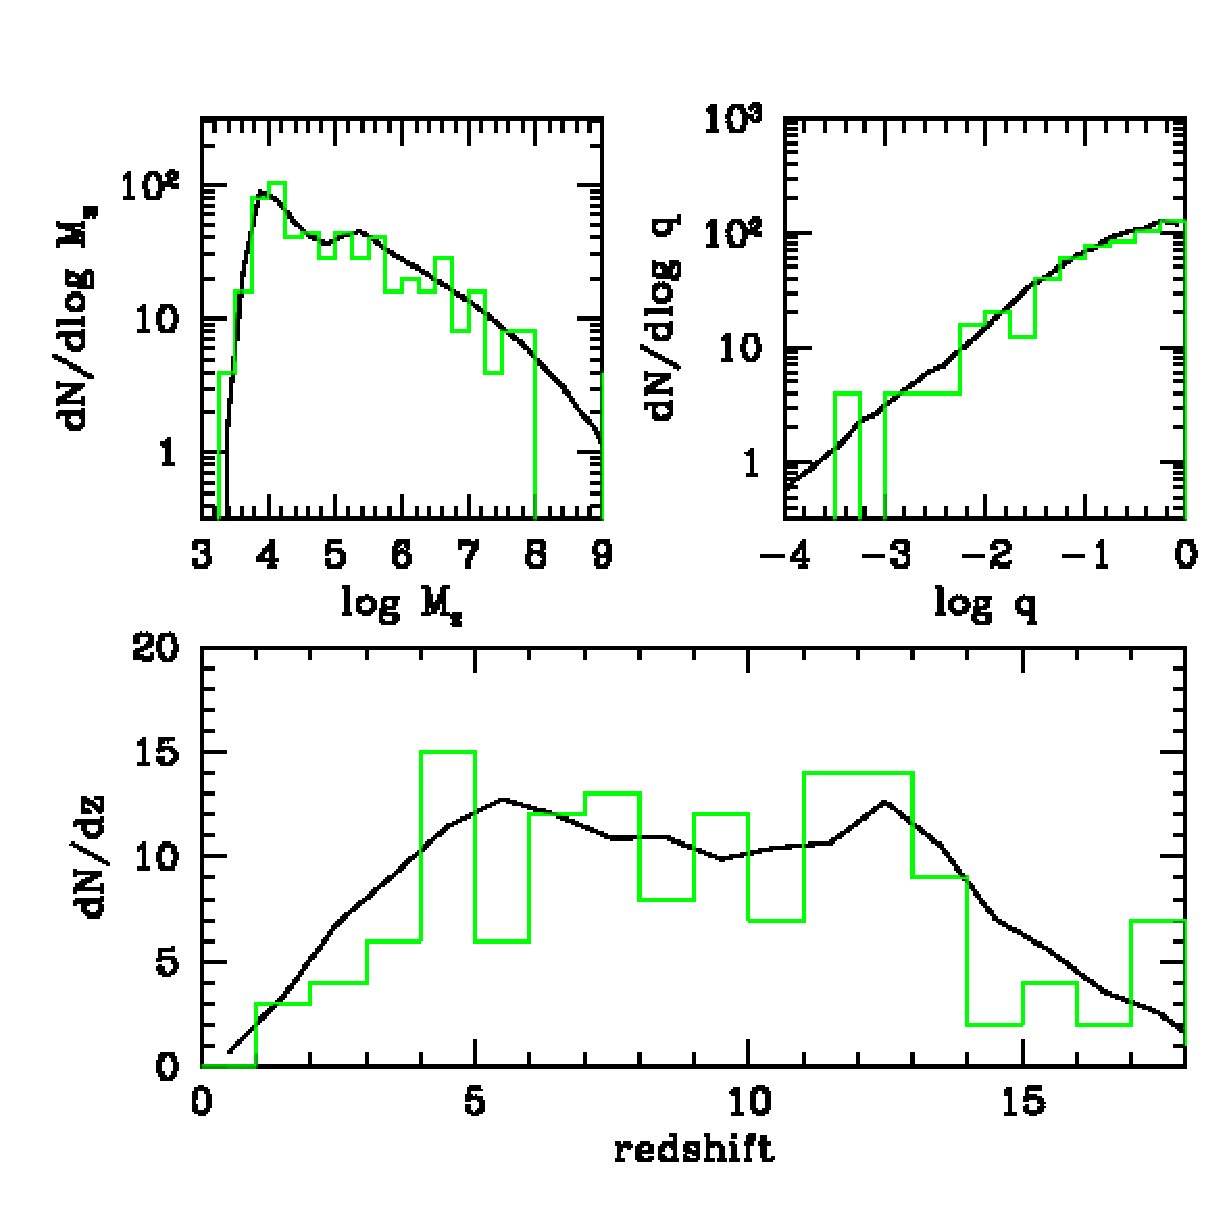
\includegraphics[width=0.65\textwidth]{FigSMBHModSel/FIG_EXAMPLE_POP.eps}
\caption{Example of marginalized $dN/dM_z$ (upper left panel), $dN/dq$ (upper right panel) and $dN/dz$ (lower panel) distributions for model HOR. In each panel, the black lines are the marginalized distributions contained in the files located in the directory 'distributions'. The green histograms are the distributions obtained by realization 1 in the file model-HOR-MCevents.OUT in the 'montecarlo-catalogues' directory.
\label{F:MBHbMod:fig1} }
\end{figure}

\begin{figure}[H]
\center
   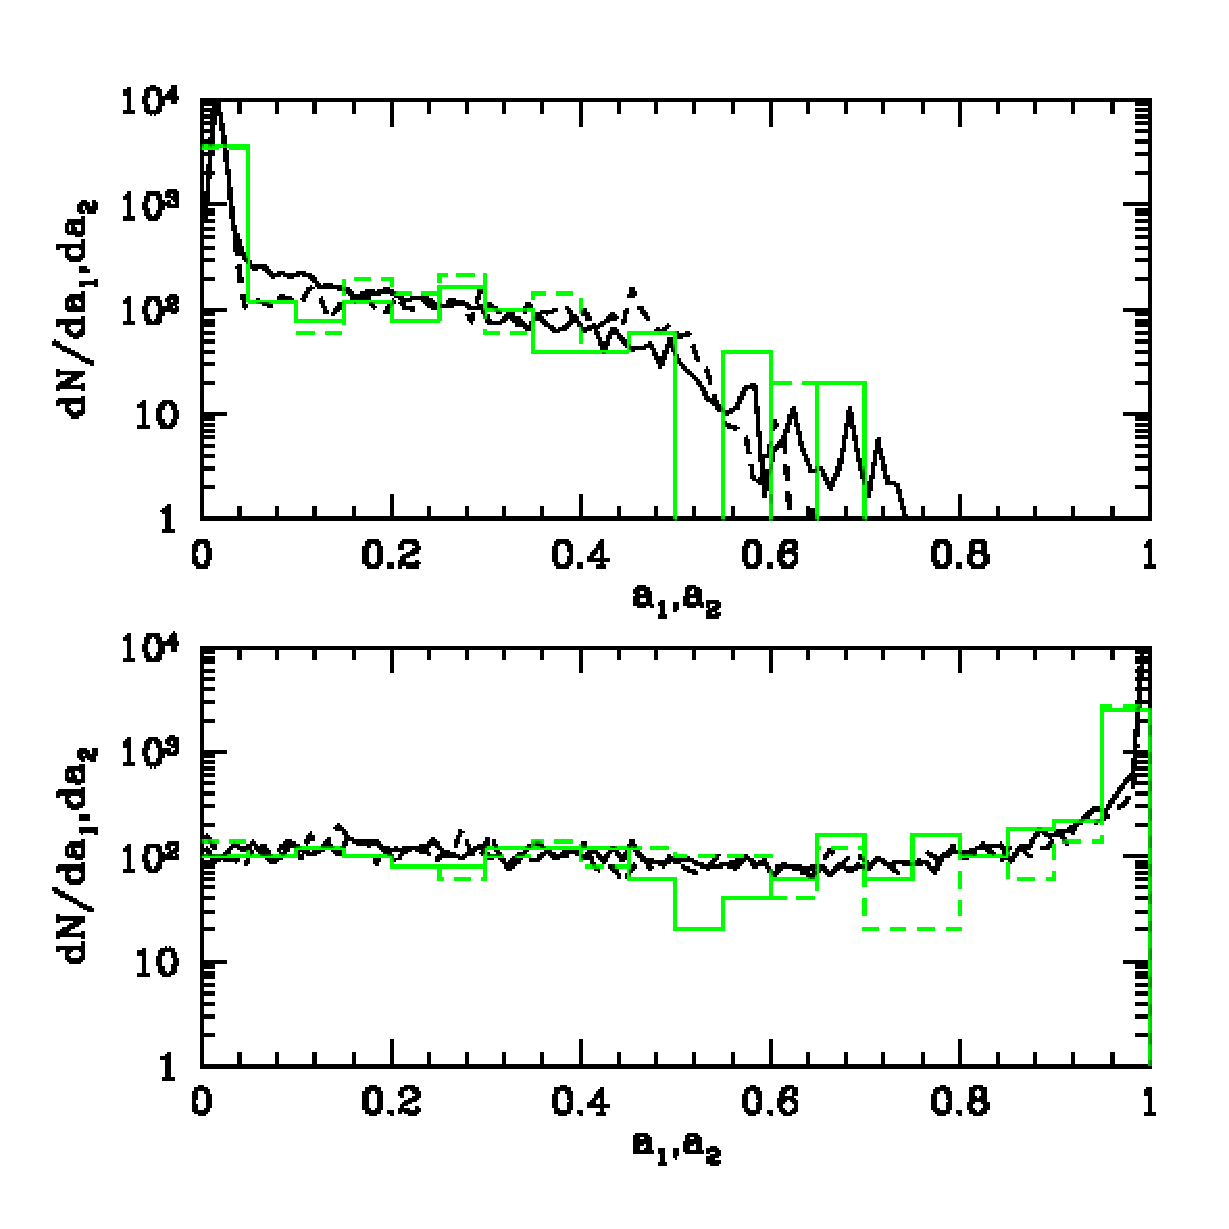
\includegraphics[width=0.65\textwidth]{FigSMBHModSel/FIG_EXAMPLE_SPINS.eps}
\caption{Example of marginalized spin distributions $dN/da_1$ (solid lines) and $dN/da_2$ (dashed lines) for models SE (VHM coherent, lower panel) and SC (VHM chaotic, upper panel). Histograms are the distributions obtained by realization 1 in the file model-SC-MCevents.OUT (upper panel) and model-SE-MCevents.OUT (lower panel) in the 'montecarlo-catalogues' directory.
\label{F:MBHbMod:fig2} } 
\end{figure}

\begin{figure}[H]
\center
   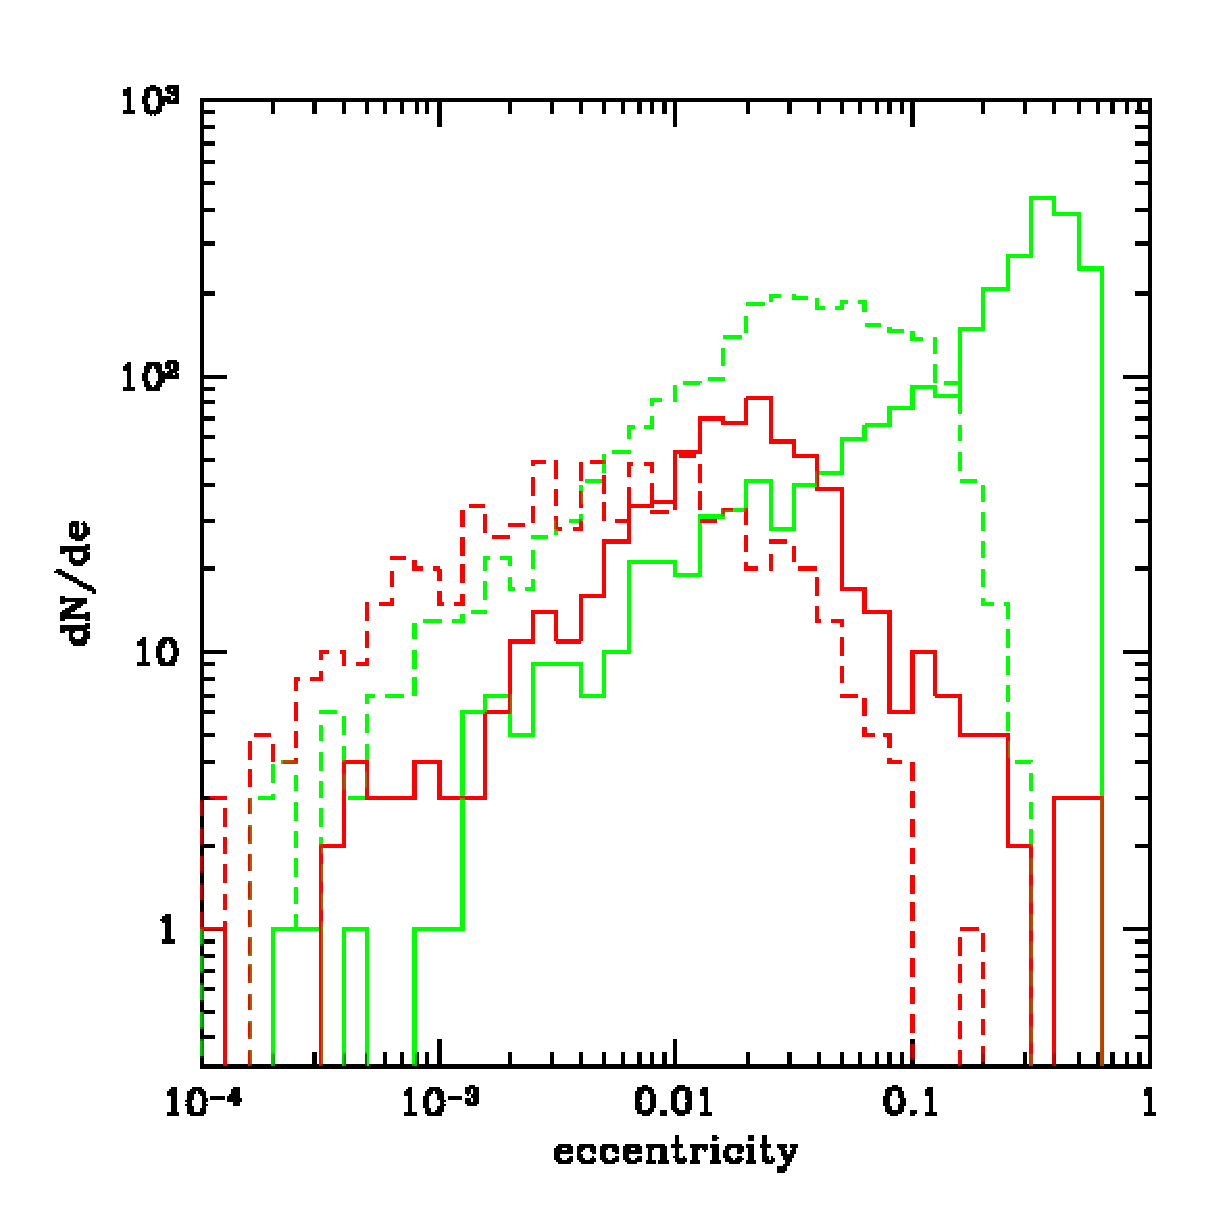
\includegraphics[width=0.65\textwidth]{FigSMBHModSel/FIG_EXAMPLE_ECCENTRICITY.eps}
\caption{Eccentricity distributions at {\it observed} gravitational wave frequency of $10^{-4}$ Hz for model SE (VHM coherent, solid green histogram), SC (VHM chaotic, dashed green histogram), LE (BVR coherent, solid red histogram), LC (BVR chaotic, dashed red histogram). Coherent models are evolved via gas dynamics, whereas star driven dynamics is assumed for the chaotic models. The distributions are obtained by averaging over the 10 Montecarlo realizations contained in the
respective model*-MCevents.OUT files in the 'montecarlo-catalogues' directory.
\label{F:MBHbMod:fig3} } 
\end{figure}








%%%%%%%%%%%%%%%     MBHb : Parameter estimation
\subsection{Parameter estimation}
\label{SS:MBHbPE}
{\it ('section captains' : Neil Cornish \& Emanuele Berti) }

\subsubsection{Averaged SNRs and horizon distances  {\it (Emanuele Berti, Neil Cornish,  \&  Stas Babak)}}
\label{SSS:MBHbPEHorizon}

Let us consider the restricted PN waveforms as computed (say) in Maggiore's
book:
%
\be
\tilde h(f)=\sqrt{\f{5}{6}}\f{{\cal M}^{5/6}f^{-7/6}}{2\pi^{2/3}D_L} e^{i\psi}
\f{2Q}{2}\,.
\ee
where we write $Q=2Q/2$ for reasons that will be apparent below. Here
%
\be
Q=\f{1+\cos^2 \iota}{2}F_+ + i \cos\iota F_\times\,.
\ee
%
The angular average of the modulus squared of $2Q$ yields
%
\be
\langle (1+\cos^2 \iota)^2 F^2_+ + 4\cos^2\iota F^2_\times
\rangle^{1/2}=\f{4}{5}\,,
\ee
%
so we get an angle-averaged Fourier amplitude of
%
\be
\tilde h(f)
=\sqrt{\f{5}{6}}\f{{\cal M}^{5/6}f^{-7/6}}{2\pi^{2/3}D_L}e^{i\psi}\f{2}{5}
=\f{1}{\sqrt{30}}\f{{\cal M}^{5/6}f^{-7/6}}{\pi^{2/3}D_L}e^{i\psi}\,.
\ee
%
which is the same as Eq.~(2.1b) in \cite{Berti:2004bd}. We multiply this by
$\f{\sqrt{3}}{2}$ to take into account the $60^\circ$ orientation of the LISA
configuration, so our starting point is Eq.~(2.1a) in \cite{Berti:2004bd}:
%
\be
\tilde h(f)
=\f{\sqrt{3}}{2}
\f{1}{\sqrt{30}}
\f{{\cal M}^{5/6}f^{-7/6}}{\pi^{2/3}D_L}e^{i\psi}\,.
\ee
%
The SNR is defined in the usual way (see e.g. Eq.~(2.6) in
\cite{Berti:2004bd}):
%
\be
\rho^2 = 4\int_{f_{\rm in}}^{f_{\rm fin}} \f{|\tilde
  h(f)|^2}{S_n^{\rm NSA}(f)} df\,,
\ee
%
where the {\it non sky-averaged} noise spectral density $S_n^{\rm NSA}(f)$ is
related to the {\it sky-averaged} (but not inclination-averaged!) noise
spectral density provided by Neil and by Shane's Sensitivity Curve Generator,
$S_n^{\rm NSA}(f)$, by
%
\be\label{noiseNSA}
S_n^{\rm NSA}(f)=\f{3}{20}S_n^{\rm SA}(f)\,.
\ee
%
Putting everything together, the integral to compute for restricted PN
inspirals is
%
\be
\rho = \sqrt{\f{2}{3}} \f{{\cal M}^{5/6}}{\pi^{2/3}D_L}
\left[
\int_{f_{\rm in}}^{f_{\rm fin}} \f{f^{-7/3}}{S_n^{\rm SA}(f)}df
\right]^{1/2}\,.
\ee
%
The SNR for phenomenological waveforms is computed following the same
conventions. For the 5/6 link configurations, these average SNRs are then
multiplied by a factor $\sqrt{2}$. In the present calculation we use the {\sc
  PhenomC} model \cite{Santamaria:2010yb}, but if needed for comparisons we
can easily compute SNRs for {\sc PhenomA} \cite{Ajith:2007kx} and {\sc
  PhenomB} \cite{Ajith:2009bn}.

Horizon distances are computed as follows: for a given cosmological model
(here $\Omega_M = 0.28$, $\Omega_\Lambda = 0.72$, $H_0 = 70$~km/s/Mpc), first
compute the SNR as a function of $M_z=M(1+z)$ at (say) $z=1$. Then use the
fact that SNR$\sim D_L^{-1}$ to find the horizon luminosity distance $D_{L,
  {\rm hor}}$ at which SNR$=10$. Finally, find the redshift $z_{\rm hor}(D_{L,
  {\rm hor}})$ corresponding to that luminosity distance by inverting
(numerically) $D_L(z)$. Horizon distances and redshifts are plotted as
functions of the mass $M$ in the {\it source} frame.

The right panel of Fig.~\ref{fig:zMiniLISA} shows that, even including merger
and ringdown, Configuration 2 is necessary to reach $z>10$ for all $M\gtrsim
10^4 M_\odot$.

%\clearpage

%%%%%%%%%%%%%%%%%%%%%%%%%%%%%%%%%%%%%%%%%%%%%%%%%%%%%%%%%%%%%%%%%%%%%%%%%%%%%%%
\section*{``Quick and dirty'' ringdown parameter estimation}
%%%%%%%%%%%%%%%%%%%%%%%%%%%%%%%%%%%%%%%%%%%%%%%%%%%%%%%%%%%%%%%%%%%%%%%%%%%%%%%

Errors on ringdown estimates of the mass and spin should be very small and
generally negligible. I propose to estimate them following \cite{Berti:2005ys}
(henceforth BCW), as follows. In the $\delta$-function or constant noise limit
we can compute the SNR as [(3.16) in BBW, where we include redshift factors
  and substitute $r$ by $D_L$ as appropriate]:
%
\beq
\label{rhoanalytic}
\rho_{\rm FH} = \left (\frac{2}{5} \right )^{1/2} 
	\left (\frac{1}{\pi {\cal F}_{lmn} D_L} \right )
	\left (\frac{\epsilon_{\rm rd}}{S_h^{\rm NSA}(f_{lmn})} \right )^{1/2}
        \left[M(1+z)\right]^{3/2}
	\frac{2Q_{lmn}}{\sqrt{1+4Q_{lmn}^2}} \,,
\eeq
%
where $M$ is the mass in the source frame. Note that this expression involves
the {\it non sky-averaged} noise curve (see expressions above). Also,
%
\beq
{\cal F}_{lmn}&=&M\omega_{lmn}=2\pi M\, f_{lmn}=f_1+f_2(1-j)^{f_3}\,,\\
Q_{lmn}&=&q_1+q_2(1-j)^{q_3}\,,
\eeq
%
where $j$ is the dimensionless spin of the final black hole, and for the
fundamental mode with $l=m=2$ we have (Table VIII):
%
$f_1=1.5251$,
$f_2=-1.1568$,
$f_3=0.1292$ and
$q_1=0.7000$,
$q_2=1.4187$,
$q_3=-0.4990$.
%
Then the errors on mass and spin, in the Flanagan-Hughes convention
\cite{Flanagan:1997sx}, can be estimated as [(4.12a), (4.12b) in BCW]:
%
%\begin{subequations}
\label{rii}
\beq
\sigma_j &=&
\frac{1}{\rho_{\rm FH}}
\left|2\frac{Q_{lmn}}{Q_{lmn}'}
\left(1+\f{1+4\beta}{16\Qlm^2}\right)\right|\,, \label{erra}\\
\f{\sigma _M}{M} &=&
\frac{1}{\rho_{\rm FH}}
\left|2\frac{Q_{lmn}
f_{lmn}'}{f_{lmn}Q_{lmn}'}
\left(1+\f{1+4\beta}{16 \Qlm^2}\right)\right|\,, \label{errm}
\eeq
%\end{subequations}
%
where a prime denotes a derivative with respect to $j$. In general we would
have
%
\be
\beta = \sin^2 \psi \cos 2\ph^\times - \cos^2 \psi \cos 2\ph^+\,
\ee
%
with 
%
$\cos \psi \equiv 1/\sqrt{1+N_\times^2}$, 
%
$\sin \psi \equiv N_\times/\sqrt{1+N_\times^2}$. 
%
The parameter $N_\times$ is the ratio between plus and cross polarization
amplitudes. If we follow Flanagan-Hughes, we can set $N_\times=1$,
$\phi^+=\phi^\times=0$, and therefore $\beta=0$, which simplifies the
expressions even further.

The only missing ingredient here is an estimate of ringdown efficiency,
$\epsilon_{\rm rd}$. I propose to use the estimate of Eq.~(4.12) in
  \cite{Berti:2007fi}:
%
\be
\epsilon_{\rm rd}=0.271\f{q^2}{(1+q)^4}\,,
\ee
%
where $q=m_1/m_2>1$ is the mass ratio of the binary. In fact, we can even use
the more optimistic ``matched-filtering based'' estimate of Eq.~(4.17) in
\cite{Berti:2007fi}:
%
\be
\epsilon_{\rm rd}=0.44\f{q^2}{(1+q)^4}\,.
\ee
%
If you want I can try to improve these estimates by including corrections due
to the spins. The ``spin expansion'' formalism of Boyle and Kesden suggests
that these corrections will be proportional to the sum of the components of
the binary spins along the orbital angular momentum. The corrections will
change $\epsilon_{\rm rd}$ by at most a factor $\approx 2$. I expect the
errors on mass and spin to be negligible anyway, so I would not bother...

%\clearpage

%%%%%%%%%%%%%%%%%%%%%%%%%%%%%%%%%%%%%%%%%%%%%%%%%%%%%%%%%%%%%%%%%%%%%%%%%%%%%%%
%\section*{Averaged SNRs and horizon distances for New LISA (5/2/2011)}
%%%%%%%%%%%%%%%%%%%%%%%%%%%%%%%%%%%%%%%%%%%%%%%%%%%%%%%%%%%%%%%%%%%%%%%%%%%%%%%

%
\begin{figure*}[H]
\begin{center}
\begin{tabular}{cc}
\includegraphics[scale=0.33,clip=true]{FigEmanuele/SNRNewLISAinsp.eps}
&\includegraphics[scale=0.33,clip=true]{FigEmanuele/SNRNewLISAIMR.eps}\\
\end{tabular}
\caption{\label{fig:SNRMiniLISA} Angle-averaged SNR for equal-mass,
  nonspinning binaries as a function of redshifted mass, $M_z=M(1+z)$. Solid
  lines: instrumental noise+galactic background; dashed lines: instrumental
  noise only.  Left: restricted PN inspiral; right: {\sc PhenomC}
  inspiral/merger/ringdown. In the right panel, thick lines refer to
  nonspinning binaries, and thin lines refer to binaries with $s_1=s_2=0.9$.}
\end{center}
\end{figure*}
%

%
\begin{figure*}[H]
\begin{center}
\begin{tabular}{cc}
\includegraphics[scale=0.33,clip=true]{FigEmanuele/zhorNewLISAinsp.eps}
&\includegraphics[scale=0.33,clip=true]{FigEmanuele/zhorNewLISAIMR.eps}\\
\end{tabular}
\caption{\label{fig:zMiniLISA} Horizon redshift $z_{\rm hor}$ (in Mpc) for
  equal-mass binaries as a function of the source mass $M$. Left: restricted
  PN inspiral; right: {\sc PhenomC} inspiral/merger/ringdown. Linestyles are
  the same as in Fig.~\ref{fig:SNRMiniLISA}.}
\end{center}
\end{figure*}
%

%
\begin{figure*}[H]
\begin{center}
\begin{tabular}{cc}
\includegraphics[scale=0.33,clip=true]{FigEmanuele/DLNewLISAinsp.eps}&
\includegraphics[scale=0.33,clip=true]{FigEmanuele/DLNewLISAIMR.eps}\\
\end{tabular}
\caption{\label{fig:DLMiniLISA} Horizon luminosity distance $D_{L, {\rm hor}}$
  (in Mpc) for equal-mass binaries as a function of the source mass $M$. Left:
  restricted PN inspiral; right: {\sc PhenomC}
  inspiral/merger/ringdown. Linestyles are the same as in
  Fig.~\ref{fig:SNRMiniLISA}.}
\end{center}
\end{figure*}
%

%
\begin{figure*}[H]
\begin{center}
\begin{tabular}{cc}
\includegraphics[scale=0.41,clip=true]{FigEmanuele/InspSNRContourz1.ps}
&\includegraphics[scale=0.41,clip=true]{FigEmanuele/IMRSNRContourz1.ps}\\
\includegraphics[scale=0.41,clip=true]{FigEmanuele/C2InspSNRContourz1.ps}
&\includegraphics[scale=0.41,clip=true]{FigEmanuele/C2IMRSNRContourz1.ps}\\
\includegraphics[scale=0.41,clip=true]{FigEmanuele/C3InspSNRContourz1.ps}
&\includegraphics[scale=0.41,clip=true]{FigEmanuele/C3IMRSNRContourz1.ps}\\
\includegraphics[scale=0.41,clip=true]{FigEmanuele/C1InspSNRContourz1.ps}
&\includegraphics[scale=0.41,clip=true]{FigEmanuele/C1IMRSNRContourz1.ps}\\
\end{tabular}
\caption{\label{fig:SNRMiniLISA2} Angle-averaged SNR for equal-mass,
  nonspinning binaries as a function of redshifted mass, $M_z=M(1+z)$.}
\end{center}
\end{figure*}
%

%
\begin{figure*}[H]
\begin{center}
\begin{tabular}{cc}
\includegraphics[scale=0.41,clip=true]{FigEmanuele/InspSNRContourz1.ps}
&\includegraphics[scale=0.41,clip=true]{FigEmanuele/IMRSNRContourz1.ps}\\
\includegraphics[scale=0.41,clip=true]{FigEmanuele/C4InspSNRContourz1.ps}
&\includegraphics[scale=0.41,clip=true]{FigEmanuele/C4IMRSNRContourz1.ps}\\
\includegraphics[scale=0.41,clip=true]{FigEmanuele/C5InspSNRContourz1.ps}
&\includegraphics[scale=0.41,clip=true]{FigEmanuele/C5IMRSNRContourz1.ps}\\
\end{tabular}
\caption{\label{fig:SNRMiniLISA3} Angle-averaged SNR for equal-mass,
  nonspinning binaries as a function of redshifted mass, $M_z=M(1+z)$.}
\end{center}
\end{figure*}
%

%
\begin{figure*}[H]
\begin{center}
\begin{tabular}{cc}
\includegraphics[scale=0.41,clip=true]{FigEmanuele/InspZhorContour.ps}
&\includegraphics[scale=0.41,clip=true]{FigEmanuele/IMRZhorContour.ps}\\
\includegraphics[scale=0.41,clip=true]{FigEmanuele/C2InspZhorContour.ps}
&\includegraphics[scale=0.41,clip=true]{FigEmanuele/C2IMRZhorContour.ps}\\
\includegraphics[scale=0.41,clip=true]{FigEmanuele/C3InspZhorContour.ps}
&\includegraphics[scale=0.41,clip=true]{FigEmanuele/C3IMRZhorContour.ps}\\
\includegraphics[scale=0.41,clip=true]{FigEmanuele/C1InspZhorContour.ps}
&\includegraphics[scale=0.41,clip=true]{FigEmanuele/C1IMRZhorContour.ps}\\
\end{tabular}
\caption{\label{fig:SNRMiniLISA4} Horizon redshift.}
\end{center}
\end{figure*}
%

%
\begin{figure*}[H]
\begin{center}
\begin{tabular}{cc}
\includegraphics[scale=0.41,clip=true]{FigEmanuele/InspZhorContour.ps}
&\includegraphics[scale=0.41,clip=true]{FigEmanuele/IMRZhorContour.ps}\\
\includegraphics[scale=0.41,clip=true]{FigEmanuele/C4InspZhorContour.ps}
&\includegraphics[scale=0.41,clip=true]{FigEmanuele/C4IMRZhorContour.ps}\\
\includegraphics[scale=0.41,clip=true]{FigEmanuele/C5InspZhorContour.ps}
&\includegraphics[scale=0.41,clip=true]{FigEmanuele/C5IMRZhorContour.ps}\\
\end{tabular}
\caption{\label{fig:SNRMiniLISA5} Horizon redshift.}
\end{center}
\end{figure*}
%

%
\begin{figure*}[H]
\begin{center}
\begin{tabular}{cc}
\includegraphics[scale=0.41,clip=true]{FigEmanuele/InspDLContour.ps}
&\includegraphics[scale=0.41,clip=true]{FigEmanuele/IMRDLContour.ps}\\
\includegraphics[scale=0.41,clip=true]{FigEmanuele/C2InspDLContour.ps}
&\includegraphics[scale=0.41,clip=true]{FigEmanuele/C2IMRDLContour.ps}\\
\includegraphics[scale=0.41,clip=true]{FigEmanuele/C3InspDLContour.ps}
&\includegraphics[scale=0.41,clip=true]{FigEmanuele/C3IMRDLContour.ps}\\
\includegraphics[scale=0.41,clip=true]{FigEmanuele/C1InspDLContour.ps}
&\includegraphics[scale=0.41,clip=true]{FigEmanuele/C1IMRDLContour.ps}\\
\end{tabular}
\caption{\label{fig:SNRMiniLISA6} Horizon luminosity distance.}
\end{center}
\end{figure*}
%

%
\begin{figure*}[H]
\begin{center}
\begin{tabular}{cc}
\includegraphics[scale=0.41,clip=true]{FigEmanuele/InspDLContour.ps}
&\includegraphics[scale=0.41,clip=true]{FigEmanuele/IMRDLContour.ps}\\
\includegraphics[scale=0.41,clip=true]{FigEmanuele/C4InspDLContour.ps}
&\includegraphics[scale=0.41,clip=true]{FigEmanuele/C4IMRDLContour.ps}\\
\includegraphics[scale=0.41,clip=true]{FigEmanuele/C5InspDLContour.ps}
&\includegraphics[scale=0.41,clip=true]{FigEmanuele/C5IMRDLContour.ps}\\
\end{tabular}
\caption{\label{fig:SNRMiniLISA7} Horizon luminosity distance.}
\end{center}
\end{figure*}
%

%
\begin{figure*}[H]
\begin{center}
\begin{tabular}{cc}
\includegraphics[scale=0.33,clip=true]{FigEmanuele/SNRinsp.eps}
&\includegraphics[scale=0.33,clip=true]{FigEmanuele/SNRIMR.eps}\\
\end{tabular}
\caption{\label{fig:SNR} Angle-averaged SNR for equal-mass, nonspinning
  binaries as a function of redshifted mass, $M_z=M(1+z)$. For the 5/6link
  configurations we multiplied the average SNR by a factor $\sqrt{2}$. Left:
  restricted PN inspiral; right: {\sc PhenomC} inspiral/merger/ringdown.}
\end{center}
\end{figure*}
%

%
\begin{figure*}[H]
\begin{center}
\begin{tabular}{cc}
\includegraphics[scale=0.33,clip=true]{FigEmanuele/DLinsp.eps}
&\includegraphics[scale=0.33,clip=true]{FigEmanuele/DLIMR.eps}\\
\end{tabular}
\caption{\label{fig:DL} Horizon luminosity distance $D_{L, {\rm hor}}$ (in
  Mpc) for equal-mass, nonspinning binaries as a function of the source mass
  $M$. Recall that for the 5/6link configurations we multiplied the average
  SNR by a factor $\sqrt{2}$. Left: restricted PN inspiral; right: {\sc
    PhenomC} inspiral/merger/ringdown.}
\end{center}
\end{figure*}
%

%
\begin{figure*}[H]
\begin{center}
\begin{tabular}{cc}
\includegraphics[scale=0.33,clip=true]{FigEmanuele/zhorinsp.eps}
&\includegraphics[scale=0.33,clip=true]{FigEmanuele/zhorIMR.eps}\\
\end{tabular}
\caption{\label{fig:z} Horizon redshift $z_{\rm hor}$ (in Mpc) for equal-mass,
  nonspinning binaries as a function of the source mass $M$. Recall that for
  the 5/6link configurations we multiplied the average SNR by a factor
  $\sqrt{2}$. Left: restricted PN inspiral; right: {\sc PhenomC}
  inspiral/merger/ringdown.}
\end{center}
\end{figure*}
%

%
\begin{figure*}[H]
\begin{center}
\includegraphics[scale=0.33,clip=true]{FigEmanuele/SNRIMRSpin09.eps}\\
\begin{tabular}{cc}
\includegraphics[scale=0.33,clip=true]{FigEmanuele/DLIMRSpin09.eps}&
\includegraphics[scale=0.33,clip=true]{FigEmanuele/zhorIMRSpin09.eps}\\
\end{tabular}
\caption{\label{fig:spin} SNR, horizon luminosity distance $D_{L, {\rm hor}}$
  (in Mpc) and horizon redshift $z_{\rm hor}$ for equal-mass, spinning
  binaries with near-maximal aligned spins (Kerr parameters
  $s_1=s_2=0.9$). SNRs and horizon distances improve slightly with respect to
  the nonspinning case, but not by orders of magnitude.}
\end{center}
\end{figure*}
%

%
\begin{figure*}[H]
\begin{center}
\includegraphics[scale=0.33,clip=true]{FigEmanuele/noise.eps}
\caption{\label{fig:PSD}
  Non-sky averaged noise spectral density, Eq.~(\ref{noiseNSA}), for Classic
  LISA and for the three New LISA configurations. Dashed lines include the
  galactic background, solid lines refer to the instrumental noise only.}
\end{center}
\end{figure*}
%

%
\begin{figure*}[H]
\begin{center}
\includegraphics[scale=0.33,clip=true]{FigEmanuele/noiseC3C5.eps}
\caption{\label{fig:PSDC3C5} Non-sky averaged noise spectral density,
  Eq.~(\ref{noiseNSA}), for Classic LISA and for New LISA C3/C5 including the
  galactic background.}
\end{center}
\end{figure*}
%










%%%%%%%%%%%%%%%%%%%%%%%%%%%%%%%%%%%%%%%%%%%%%%%%%%%%%%%%%%%%%%%%%%%%%%%
%%%%%%%%%%%%%%%%%%%%%%%%%%%%%%%%%%%%%%%%%%%%%%%%%%%%%%%%%%%%%%%%%%%%%%%
\subsubsection{Results using inspiral waveform with spin precession and higher harmonics  {\it (Ryan Lang \& Neil Cornish)}}
\label{SSS:MBHbPEInspPrecHHRyan}


Preliminary results for parameter estimation with spin precession and higher harmonics
Sources: LC and SC catalogs, requiring SNR $> 8$ (6 link case), 3 months $< t_c < $ 2 years, mass ratio $< 50$.  (SCClassic and SCConfig4 are not quite done but have more viable sources than the other cases.)

\begin{figure}[H]
\includegraphics[scale=0.54]{FigSMBHRyanNeil/LCm13.eps}
\includegraphics[scale=0.54]{FigSMBHRyanNeil/LCm14.eps}
\includegraphics[scale=0.54]{FigSMBHRyanNeil/SCm13.eps}
\includegraphics[scale=0.54]{FigSMBHRyanNeil/SCm14.eps}
\caption{Mass error}
\end{figure}

\begin{figure}[H]
\includegraphics[scale=0.54]{FigSMBHRyanNeil/LCchi13.eps}
\includegraphics[scale=0.54]{FigSMBHRyanNeil/LCchi14.eps}
\includegraphics[scale=0.54]{FigSMBHRyanNeil/SCchi13.eps}
\includegraphics[scale=0.54]{FigSMBHRyanNeil/SCchi14.eps}
\caption{Spin error}
\end{figure}

\begin{figure}[H]
\includegraphics[scale=0.54]{FigSMBHRyanNeil/LCD3.eps}
\includegraphics[scale=0.54]{FigSMBHRyanNeil/LCD4.eps}
\includegraphics[scale=0.54]{FigSMBHRyanNeil/SCD3.eps}
\includegraphics[scale=0.54]{FigSMBHRyanNeil/SCD4.eps}
\caption{Distance error}
\end{figure}

\begin{figure}[H]
\includegraphics[scale=0.54]{FigSMBHRyanNeil/LC2a3.eps}
\includegraphics[scale=0.54]{FigSMBHRyanNeil/LC2a4.eps}
\includegraphics[scale=0.54]{FigSMBHRyanNeil/SC2a3.eps}
\includegraphics[scale=0.54]{FigSMBHRyanNeil/SC2a4.eps}
\caption{Sky position major axis (degrees)}
\end{figure}


%%%%%%%%%%%%%%%%%%%%%%%%%%%%%%%%%%%%%%%%%%%%%%%%%%%%%%%%%%%%%%%%%%%%%%%
%%%%%%%%%%%%%%%%%%%%%%%%%%%%%%%%%%%%%%%%%%%%%%%%%%%%%%%%%%%%%%%%%%%%%%%
\subsubsection{Results using inspiral waveform with spin precession and higher harmonics  {\it (Antoine Petiteau, Sofiane Aoudia \& Stas Babak)}}
\label{SSS:MBHbPEInspAEI}




%%%%%%%%%%%%%%%%%%%%%%%%%%%%%%%%%%%%%%%%%%%%%%%%%%%%%%%%%%%%%%%%%%%%%%%
%%%%%%%%%%%%%%%%%%%%%%%%%%%%%%%%%%%%%%%%%%%%%%%%%%%%%%%%%%%%%%%%%%%%%%%
\subsubsection{Inspiral-Merger-Ringdown with higher harmonics (EOB based)  {\it (Sean McWilliams)}}
\label{SSS:MBHbPEPhenomAEI}



%%%%%%%%%%%%%%%%%%%%%%%%%%%%%%%%%%%%%%%%%%%%%%%%%%%%%%%%%%%%%%%%%%%%%%%
%%%%%%%%%%%%%%%%%%%%%%%%%%%%%%%%%%%%%%%%%%%%%%%%%%%%%%%%%%%%%%%%%%%%%%%
\subsubsection{Results using inspiral waveform with higher harmonics  {\it (Ed Porter)}}
\label{SSS:MBHbPEInspHHEd}


%%%%%%%%%%%%%%%%%%%%%%%%%%%%%%%%%%%%%%%%%%%%%%%%%%%%%%%%%%%%%%%%%%%%%%%
%%%%%%%%%%%%%%%%%%%%%%%%%%%%%%%%%%%%%%%%%%%%%%%%%%%%%%%%%%%%%%%%%%%%%%%
\subsubsection{Results using ringdown phase  {\it (Ioannis Kamaretsos, B.Sathyaprakash)}}
\label{SSS:MBHbPERingdown}


%%%%%%%%%%%%%%%%%%%%%%%%%%%%%%%%%%%%%%%%%%%%%%%%%%%%%%%%%%%%%%%%%%%%%%%
%%%%%%%%%%%%%%%%%%%%%%%%%%%%%%%%%%%%%%%%%%%%%%%%%%%%%%%%%%%%%%%%%%%%%%%
\subsubsection{Results using PhenomC (Inspiral-Merger-Ringdown) from AEI {\it (Stas Babak, Antoine Petiteau, Alberto Sesana, Frank Ohme \& Emma Robinson)}}
\label{SSS:MBHbPEPhenomAEI}
We use PhenomC waveforms described in \cite{Santamaria:2010yb}. Waveforms include merger and ringdown and assume aligned spins. Given the latter assumption, we apply them to efficient accretion models (SE, LE) only. Moreover, since the waveforms can not handle too extreme cases, we lower the maximal spin limit to 0.98, and considered only sources with mass ratio larger than $q=M_2/M_1=0.05$, thus loosing 10-20\% of the sources (depending on the MBH population model) in our analysis. The waveform is designed only for a dominant (2,2) harmonic and $h_{+}, h_{x}$ are
generated in the frequency domain. We have used rigid-adiabatic approximation to the TDI response (1st generation). For the inspiral part 
we have considered the spacecraft motion by using the correspondence (via  stationary phase  approximation) between frequency of the GW signal 
and the time. However this relationship becomes not applicable as we approach the merger (we use monotonous increase in time and in frequency
as validity condition).  For the merger and the ringdown (less than few days) we have assumed the static LISA. This simplified assumption 
does not affect SNR estimation but might overestimate (slightly) the error for the sky location. Some information about the sky location 
comes from the triangulation (at high frequency) as GW signal propagates across the constellation, and other information is due to modulation of the 
amplitude through antenna pattern and Dopper modulation of the phase. Assumption of the static LISA removes the modulation of the signal.
For the halo orbit around L1 we have used the numerical orbit and assuming adiabatic evolution of the GW signal.

We consider a threshold SNR$=6$ for detection, and SNR$=10$ for trustworthy parameter estimations. We show results for detectors LISA, halo L1, C4, C5, C2, C3 and C5,  assuming a single Michelson interferometer. 

First we consider the detection abilities of different configurations for that we have considered all realizations and sources from 
the ``{\bf HOR}'' catalog  described earlier in the section 3.1. The LISA and C2 configurations are given in the figures \ref{LISA_mc_SNR},
 \ref{C2_mc_SNR} below.  In all these figures the horizontal axis is the redshift. The top panel shows the average SNR for a given 
 configuration (black circles) upper and lower triangles show the dispersion (one sigma). The second panel from the top gives an 
 average over realizations fraction of the  detected events with one sigma error bar. This plot has to be read together with the lower panel
 which gives the average number of detectable events (third panel from the top). The last (bottom) panel gives the accumulative number of the 
 detected events with the legend providing the average number of the events observed up to redshift 5 and the total.



\begin{figure}[H]
\center
   \includegraphics[width=1\textwidth]{FigSMBHPhenomAEI/LISA_mc_SNRs.eps}
\caption{LISA performances as a function of redshift. From the top to the bottom we plot the average source SNR, the fraction of detectable sources (SNR$>6$), the mean number of detected sources, and the cumulative number of detected sources. Error bars are standard deviations; SE population model is assumed.
\label{LISA_mc_SNR} } 
\end{figure}


%\begin{figure}[H]
%\center
%   \includegraphics[width=1\textwidth]{FigSMBHPhenomAEI/C3_mc_SNRs.eps}
%\caption{Same as figure \ref{LISA_mc_SNR} but for C3.
%\label{C3_mc_SNR} } 
%\end{figure}


\begin{figure}[H]
\center
   \includegraphics[width=1\textwidth]{FigSMBHPhenomAEI/C2_mc_SNRs.eps}
\caption{Same as figure \ref{LISA_mc_SNR} but for C2.
\label{C2_mc_SNR} } 
\end{figure}


%\begin{figure}[H]
%\center
%   \includegraphics[width=1\textwidth]{FigSMBHPhenomAEI/C1_mc_SNRs}
%\caption{Same as figure \ref{LISA_mc_SNR} but for C1.
%\label{C1_mc_SNR} } 
%\end{figure}




%%%%%%%%%%%%%%%%%%%%%%%%%%%%%%%%%%%%%%%%%%%%%%%%%

The next set of figures corresponds to the results of the parameter estimation. We have used the Fisher information matrix 
to estimate expected errors. We have computed derivatives numerically. The results quoted below are obtained only for a single
Michelson (X) interferometer. Note that the PhenomC waveform possesses all parameter degeneracies as restricted PN 
model for the inspiral because it uses only the dominant harmonic, therefore the result for the sky location and for the 
distance measurement is so poor. It is known that including the higher harmonics and spin precession improves the 
result obtained here. However, the fact that we include merger and ringdown helps to have larger SNR  and  propagates the signal 
to the higher frequencies. Adding modulation of the signal due to spin-orbital coupling and higher harmonics allows 
to measure of polarization and breaks degeneracies in the parameter space (but does not add much to SNR). So these results 
have to be combined with estimates obtained from the inspiral only and interpolated to the case where we have both 
higher harmonics spin modulation and the merger-ring-down. 

The first set of figures gives the overall histograms for the error distribution for two population (for all realizations). 
All histograms give the relative errors. The tow populations used are {\bf LE} for the large seed and efficient accretion 
(spins always assumed aligned)  and {\bf SE} for small seeds and efficient accretion.

Figures \ref{Hist_SE_LISAC2C4C5} ({\bf SE} model)   and \ref{Hist_LE_LISAC2C4C5} ({\bf LE} model) compare LISA (magenta)
with C2 (blue), C4 (green) and C5 (red).  Only sources with SNR$>10$ are included. 

%%%%%%%%%%%%%%%%  Histogram LISA, C2, C4 and C5  %%%%%%%%%%%%%%%%

\begin{figure}[H]
\center
   \includegraphics[width=1\textwidth]{FigSMBHPhenomAEI/Hist_SE_LISAC2C4C5.eps}
\caption{1-$\sigma$ errors on source parameters: redshifted mass (upper left); symmetric mass ratio (upper right); spin parameter (lower left); luminosity distance (lower right). Histograms collect all the events in the SE catalogue (small seed), with SNR$>10$. Ligth blue histograms are for LISA, blue histograms are for C2, green histograms are for C4 and red histograms are for C5.
\label{Hist_SE_LISAC2C4C5} } 
\end{figure}

\begin{figure}[H]
\center
   \includegraphics[width=1\textwidth]{FigSMBHPhenomAEI/Hist_LE_LISAC2C4C5.eps}
\caption{1-$\sigma$ errors on source parameters. Similar as \ref{Hist_SE_LISAC2C4C5} with LE catalogue (large seed).
\label{Hist_LE_LISAC2C4C5} } 
\end{figure}


%%%%%%%%%%%%%%%%%%%%%%%%%%%%%%%%%%%%%%%%%%%%%%%%%%%%%%%%%%


In the next set of figures we show the degradation of the performance with the redshift. There we present the median over the 
realizations value versus the redshift. In the figures \ref{MedianSNR_SE_LISAC2C4C5} ({\bf SE} model) and in 
\ref{MedianSNR_LE_LISAC2C4C5} ({\bf LE} model) we compare again LISA, C2, C4 and C5 with the same color-coding as 
in the figures with histograms



The median source SNR with LISA, C2, C4 and C5 as a function of redshift is shown in figures \ref{MedianSNR_SE_LISAC2C4C5}-to-\ref{MedianSNR_LE_LISAC2C4C5}.

%%%%%%%%%%%%%%%%  Median errors LISA, C2, C4 and C5  %%%%%%%%%%%%%%%%

\begin{figure}[H]
\center
   \includegraphics[width=\textwidth]{FigSMBHPhenomAEI/MedianErrs_SE_LISAC2C4C5.eps}
\caption{Median 1-$\sigma$ errors on the source parameters as a function of 
$z$: redshifted mass (upper left); symmetric mass ratio (upper right); spin parameter (middle left); sky location in deg$^2$ (middle right); coalescence time in seconds (lower left); luminosity distance (lower right). Colorstyle as in figure \ref{Hist_SE_LISAC2C4C5} : ligth blue histograms are for LISA, blue histograms are for C2, green histograms are for C4 and red histograms are for C5. Model SE (small seeds) is assumed.
\label{MedianErrs_SE_LISAC2C4C5} } 
\end{figure}

\begin{figure}[H]
\center
   \includegraphics[width=1\textwidth]{FigSMBHPhenomAEI/MedianErrs_LE_LISAC2C4C5.eps}
\caption{Same as figure \ref{MedianErrs_SE_LISAC2C4C5} but for the LE (large seed) catalogue.
\label{MedianErrs_LE_LISAC2C4C5} } 
\end{figure}


Those curves are not smooth at low and high redshifts. The low redshift end has only few events and observed 
outliers are effect of low statistic.  For high redshift events we again do not have many event but due to low SNR. 
We also provide the median SNR for {\bf LE} and {\bf SE} models (with the same color-codding)  in the figures 
\ref{MedianSNR_LE_LISAC2C4C5}, \ref{MedianSNR_SE_LISAC2C4C5}.


%\vspace{1cm}

%For comparison we also add results comparing about C1, C2 and LISA and SNR for C3 : 

%Figures \ref{LISA_mc_SNR}, \ref{C3_mc_SNR}, \ref{C2_mc_SNR} and \ref{C1_mc_SNR} show the performances of LISA, C2 and C1 respectively, assuming the SE MBH binary population model.



%Figures \ref{Hist_SE_LISAC1C2} and \ref{Hist_LE_LISAC1C2} show histograms of parameter estimation accuracy for the ten realizations of model SE and LE respectively; only sources with SNR$>10$ are included. 
 

%The median source SNR and parameter estimation accuracy as a function of redshift is shown in figures 


%%%%%%%%%%%%%%%%  Median SNR LISA, C2, C4 and C5  %%%%%%%%%%%%%%%%


\begin{figure}[H]
\center
   \includegraphics[width=0.8\textwidth]{FigSMBHPhenomAEI/MedianSNR_SE_LISAC2C4C5.eps}
\caption{Median SNR s as a function of  $z$. Colorstyle as in figure \ref{Hist_SE_LISAC2C4C5} : ligth blue histograms are for LISA, blue histograms are for C2, green histograms are for C4 and red histograms are for C5. Model SE (small seeds) is assumed.
\label{MedianSNR_SE_LISAC2C4C5} } 
\end{figure}

\begin{figure}[H]
\center
   \includegraphics[width=0.8\textwidth]{FigSMBHPhenomAEI/MedianSNR_LE_LISAC2C4C5.eps}
\caption{Same as figure \ref{MedianSNR_SE_LISAC2C4C5} but for the LE (large seed) catalogue.
\label{MedianSNR_LE_LISAC2C4C5} } 
\end{figure}


%%%%%%%%%%%%%%%%  SNR vs z LISA, C1 and C3  %%%%%%%%%%%%%%%%


%%%%%%%%%%%%%%%%  Histogram LISA, C1 and C3  %%%%%%%%%%%%%%%%


%\begin{figure}[H]
%\center
%   \includegraphics[width=1\textwidth]{FigSMBHPhenomAEI/Hist_SE_LISAC1C2.eps}
%\caption{1-$\sigma$ errors on source parameters: redshifted mass (upper left); symmetric mass ratio (upper right); spin parameter (lower left); luminosity distance (lower right). Histograms collect all the events in the SE catalogue, with SNR$>10$. Red histograms are for LISA, green histograms are for C2 and blue histograms are for C1.
%\label{Hist_SE_LISAC1C2} } 
%\end{figure}



%\begin{figure}[H]
%\center
%   \includegraphics[width=1\textwidth]{FigSMBHPhenomAEI/Hist_LE_LISAC1C2.eps}
%\caption{Same as figure \ref{Hist_SE_LISAC1C2} but for the LE catalogue.
%\label{Hist_LE_LISAC1C2} } 
%\end{figure}


%%%%%%%%%%%%%%%%  Median erroe LISA, C1 and C3  %%%%%%%%%%%%%%%%


%\begin{figure}[H]
%\center
%   \includegraphics[width=0.8\textwidth]{FigSMBHPhenomAEI/MedianSNR_SE_LISAC1C2.eps}
%\caption{Median source SNR as a function of $z$. Colorstyle as in figure
%\ref{Hist_SE_LISAC1C2}. Model SE is assumed.
%\label{MedianSNR_SE_LISAC1C2} } 
%\end{figure}


%\begin{figure}[H]
%\center
%   \includegraphics[width=\textwidth]{FigSMBHPhenomAEI/MedianErrs_SE_LISAC1C2.eps}
%\caption{Median 1-$\sigma$ errors on the source parameters as a function of 
%$z$: redshifted mass (upper left); symmetric mass ratio (upper right); spin parameter (middle left); sky location in deg$^2$ (middle right); coalescence time in seconds (lower left); luminosity distance (lower right). Colorstyle as in figure \ref{fig4}. Model SE is assumed.
%\label{MedianErrs_SE_LISAC1C2} } 
%\end{figure}

%\begin{figure}[H]
%\center
%   \includegraphics[width=0.8\textwidth]{FigSMBHPhenomAEI/MedianSNR_LE_LISAC1C2.eps}
%\caption{Same as figure \ref{MedianErrs_SE_LISAC1C2} but for the LE catalogue.
%\label{MedianSNR_LE_LISAC1C2} } 
%\end{figure}

%\begin{figure}[H]
%   \includegraphics[width=\textwidth]{FigSMBHPhenomAEI/MedianErrs_LE_LISAC1C2.eps}
%\caption{Same as figure \ref{MedianErrs_SE_LISAC1C2} but for the LE catalogue.
%\label{MedianErrs_LE_LISAC1C2} } 
%\end{figure}






%%%%%%%%%%%%%%%%%%%%%%%%%%%%%%%%%%%%%%%%%%%%%%%%%%%%%%%%%%%%%%%%%%%%%%%
%%%%%%%%%%%%%%%%% Alberto comparaison 4 vs 6 links
%%%%%%%%%%%%%%%%%%%%%%%%%%%%%%%%%%%%%%%%%%%%%%%%%%%%%%%%%%%%%%%%%%%%%%%
\subsection{4 vs 6 links and low frequency sensitivity impact on the source distance determination {\it (A. Sesana)} }
\label{SS:SMBH4vs6link}


This note is a (I hope useful) followup on the discussion we had yesterday about the impact of the number of links and of the low frequency sensitivity on the source distance (redshift) determination. In each plot I show separately the impact of both, in the attempt of assessing their relative importance. I used the Horizon catalogue, which is a mix of our four 'fiducial' models, and I show histograms with the number of detected sources, averaged over 1000 realizations of the MBH binary population. The errors are computed using inspiral 2PN waveforms, and then rescaled appropriately to account for the increased SNR provided by the merger and ringdown. This is very rough, but the results have been shown by Stas to be consistent with those obtained with PhenomC waveforms. In figure \ref{F:SMBH4vs6link:fig1} I show the effect on the overall detectable population, assuming a threshold SNR$=8$ (the number of sources therefore is different for each of the configurations). In the top panel I show the progression {\bf LISA 6 links $\rightarrow$ LISA 4 links $\rightarrow$ C2 4 links}; in the bottom panel, instead, I show {\bf LISA 6 links $\rightarrow$ C2 6 links $\rightarrow$ C2 4 links}. In general, both reducing the low frequency sensitivity (i.e. reducing the time spent in band by the source) and cutting 2 links (i.e. losing the capability of reconstructing the two polarizations 'right away') cause a degradation in the redshift (converted from the luminosity distance using standard cosmology) determination of a factor of $\sim5$, in the relevant error range (i.e. error$<100\%$). In figure \ref{F:SMBH4vs6link:fig2} I select sources with total redshifted mass $>10^6$M$_\odot$. In this case, both factors contribute to the degradation, with a mild predominance of the low frequency reduced sensitivity. This is because such sources would be observable for a long time during their inspiral, in the LISA configuration, and we loose all that information with the descoped designs. For the low mass sources (total redshifted mass $<10^5$M$_\odot$), the switch to 4 links seems instead to be more catastrophyc. This is because, with the LISA designed, most of the inspiral of such sources is hidden in the galactic binary confusion noise, and descoping the low frequency sensitivity of the instrument doesn't affect the distance determination too much (compare in particular the black and green curve in the lower panel). Most of the degradation is therefore given by the loss of the polarization information in this case (this is actually different to what we naively thought yesterday).

Note that a C2 configuration with 6 links still gives a useful redshift determination for most of the sources, while the 4 links configuration does not (in particular for light sources at redshift $>5$, see red histograms in figure \ref{F:SMBH4vs6link:fig3}). So, in this respect, keeping 6 links would be important. 

LISA gives us distance information through: {\bf (i) constellation motion during the inspiarl phase; (ii) polarization reconstruction with the 6 links}. In the 4 links descoped baselines we loose both. So, if with LISA we could get important distance information with relatively cheap waveforms, we can not say the same with the descoped versions.

The information can be restored by including higher harmonics, eccentricity, and spin precession. However their impact has to be properly quantify. Moreover, as Gerard and Stas pointed out, {\bf our ability to determine the source distance is not anymore 'detector dependent' but 'waveform dependent'}, which is, in any case, a risk. For example, if most of the sources have almost perfectly aligned spins, even with the correct waveforms given by Mother Nature, we might not be able to determine the distance of most of them with a 4 links descoped detector; conversely we would be able to do so anyway, with a 6 links LISA-like baseline.

 
\begin{figure}[H]
\center
   \includegraphics[width=0.65\textwidth]{FigSMBHModSel/FIG_comparison_all.eps}
\caption{Redshift determination accuracy over all the observable population.
Histograms are averaged over 1000 realizations of the horizon models. Legend 
is given in the panels.
\label{F:SMBH4vs6link:fig1} } 
\end{figure}

\begin{figure}[H]
\center
   \includegraphics[width=0.65\textwidth]{FigSMBHModSel/FIG_comparison_massive.eps}
\caption{Same as figure \ref{F:SMBH4vs6link:fig1}, but for massive sources only.
\label{F:SMBH4vs6link:fig2} } 
\end{figure}

\begin{figure}[H]
\center
   \includegraphics[width=0.65\textwidth]{FigSMBHModSel/FIG_comparison_light.eps}
\caption{Same as figure \ref{F:SMBH4vs6link:fig1}, but for light sources only.
\label{F:SMBH4vs6link:fig3} } 
\end{figure}



%%%%%%%%%%%%%%%%%%%%%%%%%%%%%%%%%%%%%%%%%%%%%%%%%%%%%%%%%%%%%%%%%%%%%%%
%%%%%%%%%%%%%%%    Model selection 
%%%%%%%%%%%%%%%%%%%%%%%%%%%%%%%%%%%%%%%%%%%%%%%%%%%%%%%%%%%%%%%%%%%%%%%
\subsection{Model selection {\it (Alberto Sesana, Marta Volonteri, Emanuele Berti, Jonathan Gair) } }
\label{SS:MBHbModel}
{\it ('section captain' : Alberto Sesana) }

\section{Model Selection}
We are performing a model selection study similar to that carried by \cite{ses11}. The results should be ready within this week. Here we just share some results about the observable massive black hole binary (MBHB) population, and some crude estimation of the errors on source parameters.

In practice we consider the four default models (SE, SC, LE, LC) and a mixed model in which we artificially mixed the SE and the LE model. 
\begin{itemize}
\item For each detector configuration (LISA, C1, C2, following the standard nomenclature) we compute the transfer function, i.e., the completeness of the detector in the ($M,q,z$) parameter space. 

\item We then filter the intrinsic distribution of merging MBHBs predicted by each model with the appropriate transfer function to produce {\it theoretically observable} distributions to be compared with observed catalogues. 

\item We then draw 1000 Montecarlo realizations of each model and simulate observations with LISA, C1 and C2 including Fisher information matrix (FIM) errors. We assume two years of observations for each detector configuration and count only sources coalescing within this timespan. In table \ref{tabI} we list the number of observable sources for each model and for each detector, assuming different performances (see table caption for details).

\item Montecarlo realizations will then be compared to the {\it theoretically observable} distributions to assess model distinguishability (to be done by Jon these days).
\end{itemize}

Both the transfer functions and the Montecarlo realizations are computed considering inspiral-merger-ringdown waveforms (IMR) in the following way. Using PhenomC waveforms, Emanuele computed the average ratio ${\cal R}=$SNR$_{\rm IMR}/$SNR$_{\rm insp}$ for sources on a grid of ($M,q,z$). However, 2PN inspiral only waveforms are currently included in our codes for computing the transfer functions and to estimate parameter errors. To compute the transfer function we therefore compute the 2PN SNR$_{\rm insp}$ of each source and we rescale it by the appropriate factor ${\cal R}$. The same we do for parameter estimation; we used 2PN inspiral waveforms only, and then we rescaled the errors by the appropriate factor ${\cal R}$. This is a very crude way to proceed, but it was the only practicable one in such a short timescale, and gives reasonable results.

\section{Observable population and crude error estimation.}
We collect here some preliminary plots.
Figure \ref{F:MBHbModel:fig1} shows the marginalized {\it theoretically observable} distributions, i.e., the intrinsic MBHB coalescence distributions filtered with the appropriate transfer function. Assuming a POPIII model (SE), we loose more than 50\% of the events going from classic LISA (black) to configuration C1. Still we have a consistent source population, and a very good chance to get some event out to redshift 11-12. Figure \ref{F:MBHbModel:fig2} represents the same distributions for a massive seed model (LE), and in this case the number of observable events is much less affected ($<20\%$). Note that the difference between considering IMR waveforms (thick--dashed) and inspiral only (thin--solid) is minor, and it affects particularly massive, unequal binaries. It turns out infact that considering the merger and ringdown mostly affect the transfer function for massive, unequal binaries, which, in our models, are subdominant.

Figure \ref{F:MBHbModel:fig3} shows error distributions for configuration C2, assuming a single interferometer and threshold SNR$=8$. Dashed histograms take into account only the inspiral, while the solid ones consider also merger and ringdown (IMR). As expected, there is a mild general improvement in all the errors, when considering IMR. Note the horrendous $\Delta{z}/z$! in this case 60\% of the sources have undetermined redshift (we compute the error on the luminosity distance and we convert it in $\Delta{z}/z$ assuming a concordance cosmology). Even though such waveforms are very simplified, and the real situation is probably going to be better than this, there is an indication that a single, descoped interferometer (4 laser links) may be insufficient to decently determine the source luminosity distance/redshift. This is shown also in figure \ref{F:MBHbModel:fig4}, where configurations C1 (red), C2 (blue) and classic LISA (black) are compared. Again we assume a single interferometer with threshold SNR$=8$. There is more than an order of magnitude degradation in the error estimation of many sources, going from LISA to C1. Notice that the error in $\Delta{z}/z$ is bad also for LISA. This is because we are considering a single interferometer. The difference between one and two interferometers is shown in figure \ref{F:MBHbModel:fig5}. Here we show classic LISA (black, lower panel) and C1 (red, upper panel), considering one (solid) and two (dashed) interferometers. The histograms are shifted to the left by about a decade, adding a second Michelson. In particular for classic LISA, the typical error is $\sim10\%$, in line with our previous results. Note that few sources (massive, nearby systems) have a $\Delta{z}/z<1\%$, because of the high SNR given by the addition of the merger and the ringdown to the signal. In the C1 case, adding a second interferometer, would at least allow redshift determination of $\sim 50\%$ of the sources. 

{\bf The code used for this model selection exercise, is a
restricted PN inspiral, non-spinning code, and it is conservative in the
sense that all effects we omitted (IMR, higher-harmonics, spin) should
help; however the SNR rescaling should partially account for these
omissions. In any case, these plots show how bad is a descoped instrument 
with a single Michelson for distance determination to the source. 
It is important to understand if the situation improves significantly
by including higher-harmonics, spin, eccentricity, etc. 
Look forward to some more sophisticated parameter estimation studies
(e.g. Neil+Ryan+Scott+Antoine K. for precession+higher harmonics in the inspiral; 
Sean and NASA Goddard for IMR+higher harmonics, and so on).}

\begin{table*}
\begin{center}
\begin{tabular}{l|c|cccc}
\hline
Model & Detector  &  1 int. SNR$=8$ & 1 int. SNR$=20$ & 2 int. SNR$=8$ & 2 int. SNR$=20$\\
\hline
   & LISA & 64.96 &     40.98 &     79.73 &     49.96\\
SE & C2   & 40.09 &     23.01 &     49.73 &     29.89\\
   & C1   & 32.40 &     17.79 &     40.66 &     23.58\\
\hline				
   & LISA & 70.64 &     46.99 &     84.76 &     56.19\\
SC & C2   & 45.63 &     27.04 &     55.50 &     34.99\\
   & C1   & 37.54 &     20.84 &     46.38 &     27.86\\
\hline				
   & LISA & 48.70 &     46.04 &     49.19 &     48.56\\
LE & C2   & 44.94 &     34.62 &     47.80 &     42.11\\
   & C1   & 41.61 &     27.50 &     46.07 &     35.88\\
\hline				
   & LISA & 42.80 &     40.47 &     43.16 &     42.43\\
LC & C2   & 38.72 &     30.47 &     41.21 &     36.00\\
   & C1   & 35.30 &     25.04 &     38.81 &     31.19\\
\hline				
\end{tabular}
\end{center}
\caption{Number of {\it theoretically observable} events in two year of observation, for the four considered models (SE, SC, LE, LC), assuming three different detectors (LISA, C2, C1). The four columns correspond to four different detector performances: a single Michelson with minimal SNR$=8$ for trustworthy parameter estimation (column 3); a single Michelson with minimal SNR$=20$ for trustworthy parameter estimation (column 4); two Michelson with minimal SNR$=8$ for trustworthy parameter estimation (column 5); two Michelson with minimal SNR$=20$ for trustworthy parameter estimation (column 6).}
\label{tabI}
\end{table*}

\begin{figure}[H]
\center
   \includegraphics[width=0.65\textwidth]{FigSMBHModSel/FIG_MODEL_SE_DIST.eps}
\caption{{\it Theoretically observable} marginalized distributions for model SE. In each panel we plot curves for LISA (black), C2 (blue) and C1 (red). Thick--dashed curves are for IMR waveforms, while thin--solid are for inspiral only. The curves are normalized so that their integrals return the number of observed events in two years. The three panels show the distributions as a function of total redshifted mass ($M_z=(M_1+M_2)(1+z)$, upper left panel), mass ratio ($q=M_2/M_1<1$, upper right panel), and redshift ($z$, lower panel).
\label{F:MBHbModel:fig1} } 
\end{figure}

\begin{figure}[H]
\center
   \includegraphics[width=0.65\textwidth]{FigSMBHModSel/FIG_MODEL_LE_DIST.eps}
\caption{Same as figure \ref{F:MBHbModel:fig1} but for model LE.
\label{F:MBHbModel:fig2} } 
\end{figure}

\begin{figure}[H]
\center
   \includegraphics[width=0.65\textwidth]{FigSMBHModSel/FIG_ERRORS_C2.eps}
\caption{1-$\sigma$ errors in the determination of the binary parameters, averaged over 1000 realizations of model LE. Here we assume configuration C2, one Michelson and threshold SNR$=8$. Dashed histograms are for inspiral only, solid ones are for IMR waveforms. 
\label{F:MBHbModel:fig3} } 
\end{figure}

\begin{figure}[H]
\center
   \includegraphics[width=0.65\textwidth]{FigSMBHModSel/FIG_ERRORS_COMPARISON_81.eps}
\caption{1-$\sigma$ errors in the determination of the binary parameters, averaged over 1000 realizations of model LE, assuming different detectors: LISA (black), C2 (blue), C1 (red). We assume one Michelson and threshold SNR$=8$
\label{F:MBHbModel:fig4} } 
\end{figure}

\begin{figure}[H]
\center
   \includegraphics[width=0.65\textwidth]{FigSMBHModSel/FIG_ERR_Z_81_82.eps} 
\caption{1-$\sigma$ errors in the determination of $z$ for LISA (black, lower panel) and C1 (red, upper panel). Solid and dashed histograms are for one and two Michelson respectively. We averaged over 1000 realizations of model LE, assuming threshold SNR$=8$. 
\label{F:MBHbModel:fig5} } 
\end{figure}


















%%%%%%%%%%%%%%%%%%%%%%%%%%%%%%%%%%%%%%%%%%%%%%%%%%%%%%%%%%%%%%%%%%%%%%%
%%%%%%%%%%%%%%%%%%%%%%%%%%%%%%%%%%%%%%%%%%%%%%%%%%%%%%%%%%%%%%%%%%%%%%%



%%%%%%%%%%%%%%%%%%%%%%%%%%%%%%%%%%%%%
%                                                            EMRIs                                                        %
%%%%%%%%%%%%%%%%%%%%%%%%%%%%%%%%%%%%%

\section{EMRIs}
{\it ('section captains' : Jon Gair \& Ed Porter) }

























\begin{thebibliography}{}

\bibitem{dhu05}
{Dhurandhar}, S.~V. and {Nayak}, K.~R. and {Koshti}, S. and {Vinet}, J.-Y. Classical and Quantum Gravity {\bf 22}, 481-487 (2005)


\bibitem{Sesana:2007sh}
  A.~Sesana, M.~Volonteri and F.~Haardt,
  %``The imprint of massive black hole formation models on the LISA data
  %stream,''
  Mon.\ Not.\ Roy.\ Astron.\ Soc.\  {\bf 377}, 1711 (2007)
  [arXiv:astro-ph/0701556].
  %%CITATION = MNRAA,377,1711;%%
%\cite{Volonteri:2002vz}
 
\bibitem{Volonteri:2002vz}
  M.~Volonteri, F.~Haardt and P.~Madau,
  %``The Assembly and Merging History of Supermassive Black Holes in
  %Hierarchical Models of Galaxy Formation,''
  Astrophys.\ J.\  {\bf 582}, 559 (2003)
  [arXiv:astro-ph/0207276].
  %%CITATION = ASJOA,582,559;%%

%\cite{Berti:2006ew}
%\bibitem{Berti:2006ew}
%  E.~Berti,
%  %``LISA observations of massive black hole mergers: event rates and issues in
%  %waveform modelling,''
%  Class.\ Quant.\ Grav.\  {\bf 23}, S785 (2006)
%  [arXiv:astro-ph/0602470].
%  %%CITATION = CQGRD,23,S785;%%


%\cite{Koushiappas:2003zn}
\bibitem{Koushiappas:2003zn}
  S.~M.~Koushiappas, J.~S.~Bullock and A.~Dekel,
  %``Massive black hole seeds from low angular momentum material,''
  Mon.\ Not.\ Roy.\ Astron.\ Soc.\  {\bf 354}, 292 (2004)
  [arXiv:astro-ph/0311487].
  %%CITATION = MNRAA,354,292;%%

%\cite{Begelman:2006db}
\bibitem{Begelman:2006db}
  M.~C.~Begelman, M.~Volonteri and M.~J.~Rees,
  %``Formation of Supermassive Black Holes by Direct Collapse in Pregalactic
  %Halos,''
  Mon.\ Not.\ Roy.\ Astron.\ Soc.\  {\bf 370}, 289 (2006)
  [arXiv:astro-ph/0602363].
  %%CITATION = MNRAA,370,289;%%

%\cite{Bardeen:1970}
\bibitem{Bardeen:1970}
  J.~M.~Bardeen,
  Nature  {\bf 226}, 64 (1970).

%\cite{Thorne:1974ve}
\bibitem{Thorne:1974ve}
  K.~S.~Thorne,
  %``Disk Accretion Onto A Black Hole. 2. Evolution Of The Hole,''
  Astrophys.\ J.\  {\bf 191}, 507 (1974).
  %%CITATION = ASJOA,191,507;%%

%\cite{King:2006uu}
\bibitem{King:2006uu}
  A.~R.~King and J.~E.~Pringle,
  %``Growing Supermassive Black Holes by Chaotic Accretion,''
  Mon.\ Not.\ Roy.\ Astron.\ Soc.\ Lett.\  {\bf 373}, L93 (2006)
  [arXiv:astro-ph/0609598].
  %%CITATION = 00482,373,L93;%%

%\cite{Berti:2008af}
\bibitem{Berti:2008af}
  E.~Berti and M.~Volonteri,
  %``Cosmological Black Hole Spin Evolution by Mergers and Accretion,''
  Astrophys.\ J.\  {\bf 684}, 822 (2008)
  [arXiv:0802.0025].

%%\cite{Rezzolla:2007rz}
%\bibitem{Rezzolla:2007rz}
%  L.~Rezzolla, E.~Barausse, E.~N.~Dorband, D.~Pollney, C.~Reisswig, J.~Seiler and S.~Husa,
%  %``On the final spin from the coalescence of two black holes,''
%  Phys.\ Rev.\  D {\bf 78}, 044002 (2008)
%  [arXiv:0712.3541 [gr-qc]].
%  %%CITATION = PHRVA,D78,044002;%%

%\cite{Bogdanovic:2007hp}
\bibitem{Bogdanovic:2007hp}
  T.~Bogdanovic, C.~S.~Reynolds and M.~C.~Miller,
  %``Alignment of the spins of supermassive black holes prior to coalescence,''
  Astrophys.\ J.\ Lett.\ {\bf 661}, 147 (2007)
  [arXiv:astro-ph/0703054].
  %%CITATION = ASTRO-PH/0703054;%%

\bibitem{dotti}
M. Dotti, M. Volonteri, A. Perego, M. Colpi, M. Ruszkowski, F. Haardt, 
  Mon.\ Not.\ Roy.\ Astron.\ Soc.\  {\bf 402}, 628 (2010).

\bibitem{cuadra}
J. Cuadra, P. J. Armitage, R. D. Alexander, M. C. Begelman, 
  Mon.\ Not.\ Roy.\ Astron.\ Soc.\  {\bf 393}, 1423 (2009).

\bibitem{roedig}
C. Roedig, M. Dotti, A. Sesana, J. Cuadra, M. Colpi,
to appear in Mon.\ Not.\ Roy.\ Astron.\ Soc.\ (2011)
  [arXiv:astro-ph/1104.3868].

\bibitem{sesana}
A. Sesana, 
  Astrophys.\ J.\  {\bf 719}, 851 (2010)
%\cite{Lacey:1993iv}
\bibitem{Lacey:1993iv}
  C.~G.~Lacey and S.~Cole,
  %``Merger rates in hierarchical models of galaxy formation,''
  Mon.\ Not.\ Roy.\ Astron.\ Soc.\  {\bf 262}, 627 (1993).
  %%CITATION = MNRAA,262,627;%%

%\cite{Press:1973iz}
\bibitem{Press:1973iz}
  W.~H.~Press and P.~Schechter,
  %``Formation of galaxies and clusters of galaxies by selfsimilar gravitational
  %condensation,''
  Astrophys.\ J.\  {\bf 187}, 425 (1974).
  %%CITATION = ASJOA,187,425;%%

%\cite{Sheth:2001dp}
\bibitem{Sheth:2001dp}
  R.~K.~Sheth and G.~Tormen,
  %``An Excursion Set Model Of Hierarchical Clustering : Ellipsoidal Collapse
  %And The Moving Barrier,''
  Mon.\ Not.\ Roy.\ Astron.\ Soc.\  {\bf 329}, 61 (2002)
  [arXiv:astro-ph/0105113].
  %%CITATION = MNRAA,329,61;%%

%\cite{Haehnelt:1994wt}
\bibitem{Haehnelt:1994wt}
  M.~G.~Haehnelt,
  %``Low frequency gravitational waves from supermassive black holes,''
  Mon.\ Not.\ Roy.\ Astron.\ Soc.\  {\bf 269}, 199 (1994)
  [arXiv:astro-ph/9405032].
  %%CITATION = MNRAA,269,199;%%

%\cite{Menou:2001hb}
\bibitem{Menou:2001hb}
  K.~Menou, Z.~Haiman and V.~K.~Narayanan,
  %``The Merger History of Supermassive Black Holes in Galaxies,''
  Astrophys.\ J.\  {\bf 558}, 535 (2001)
  [arXiv:astro-ph/0101196].
  %%CITATION = ASJOA,558,535;%%

%\cite{Berti:2004bd}
\bibitem{Berti:2004bd}
  E.~Berti, A.~Buonanno, C.~M.~Will,
  %``Estimating spinning binary parameters and testing alternative theories of gravity with LISA,''
  Phys.\ Rev.\  {\bf D71}, 084025 (2005).
  [gr-qc/0411129].

%\cite{Santamaria:2010yb}
\bibitem{Santamaria:2010yb}
  L.~Santamaria, F.~Ohme, P.~Ajith, B.~Bruegmann, N.~Dorband, M.~Hannam, S.~Husa, P.~Mosta {\it et al.},
  %``Matching post-Newtonian and numerical relativity waveforms: systematic errors and a new phenomenological model for non-precessing black hole binaries,''
  Phys.\ Rev.\  {\bf D82}, 064016 (2010).
  [arXiv:1005.3306 [gr-qc]].

%\bibitem{sm10}
%L. Santamaria, F. Ohme, P. Ajith, B. Bruegmann, N. Dorband, M. Hannam, S. Husa, P. Moesta, D. Pollney, C. Reisswig, E. L. Robinson, J. Seiler and B. Krishnan,  Phys.\ Rev.\  D {\bf 82}, 064016 (2010)


%\cite{Ajith:2007kx}
\bibitem{Ajith:2007kx}
  P.~Ajith, S.~Babak, Y.~Chen, M.~Hewitson, B.~Krishnan, A.~M.~Sintes, J.~T.~Whelan, B.~Bruegmann {\it et al.},
  %``A Template bank for gravitational waveforms from coalescing binary black holes. I. Non-spinning binaries,''
  Phys.\ Rev.\  {\bf D77}, 104017 (2008).
  [arXiv:0710.2335 [gr-qc]].

%\cite{Ajith:2009bn}
\bibitem{Ajith:2009bn}
  P.~Ajith, M.~Hannam, S.~Husa, Y.~Chen, B.~Bruegmann, N.~Dorband, D.~Muller, F.~Ohme {\it et al.},
  %``Inspiral-merger-ringdown waveforms for black-hole binaries with non-precessing spins,''  
  [arXiv:0909.2867 [gr-qc]].

%\cite{Berti:2005ys}
\bibitem{Berti:2005ys}
  E.~Berti, V.~Cardoso, C.~M.~Will,
  %``On gravitational-wave spectroscopy of massive black holes with the space interferometer LISA,''
  Phys.\ Rev.\  {\bf D73}, 064030 (2006).
  [gr-qc/0512160].

%\cite{Flanagan:1997sx}
\bibitem{Flanagan:1997sx}
  E.~E.~Flanagan, S.~A.~Hughes,
  %``Measuring gravitational waves from binary black hole coalescences: 1. Signal-to-noise for inspiral, merger, and ringdown,''
  Phys.\ Rev.\  {\bf D57}, 4535-4565 (1998).
  [gr-qc/9701039].

%\cite{Berti:2007fi}
\bibitem{Berti:2007fi}
  E.~Berti, V.~Cardoso, J.~A.~Gonzalez, U.~Sperhake, M.~Hannam, S.~Husa, B.~Bruegmann,
  %``Inspiral, merger and ringdown of unequal mass black hole binaries: A Multipolar analysis,''
  Phys.\ Rev.\  {\bf D76}, 064034 (2007).
  [gr-qc/0703053 [GR-QC]].

\end{thebibliography}{}






\end{document}



